\documentclass[12pt, a4paper]{extarticle}
\usepackage{polyglossia}
\setmainlanguage{russian}

\usepackage{fontspec}
% \defaultfontfeatures{Renderer=Basic,Ligatures={TeX}}
\setmainfont{CMU Serif}
\setsansfont{CMU Sans Serif}
\setmonofont{CMU Typewriter Text}
\usepackage[utf8]{inputenc}
\usepackage{indentfirst}
\usepackage[pdfversion=1.7]{hyperref}
\usepackage{amsthm}
\usepackage{amsmath}
\usepackage{listing}
\usepackage{pdfpages}
\usepackage[pipeTables,tableCaptions]{markdown}
\usepackage{hyphenat}
\usepackage{emoji}
\usepackage[inline]{enumitem}
\usepackage[margin=15mm]{geometry}
\usepackage{longtable}
\usepackage{array,calc}
\usepackage{booktabs}
\usepackage{color}
\usepackage{tabularray}
\usepackage{minted}

\newlist{enuminl}{enumerate*}{1}
\setlist[enuminl]{label=(\arabic*)}
\newcommand{\itembf}[1]{\item \textbf{#1}}

\newcommand\tab{\par\hspace{2em}}

\author{
  Забережный Тимофей \\
  Багаев     Леонид  \\
  Москалёв   Никита  \\
  Буховец    Устин   \\
}
\title{Ответы по ОАиПу. Семестр 1}

\begin{document}
\clearpage\maketitle
\thispagestyle{empty}

\newpage
\tableofcontents
\newpage

% \markdownInput{1-18/markdown/1.md}
% \markdownInput{1-18/markdown/2.md}
% \markdownInput{1-18/markdown/3.md}
% \markdownInput{1-18/markdown/4.md}
% \markdownInput{1-18/markdown/5.md}
% \markdownInput{1-18/markdown/6.md}
% \markdownInput{1-18/markdown/7.md}
% \markdownInput{1-18/markdown/8.md}
% \markdownInput{1-18/markdown/9.md}
% \markdownInput{1-18/markdown/10.md}
% \markdownInput{1-18/markdown/11.md}
% \markdownInput{1-18/markdown/12.md}
% \markdownInput{1-18/markdown/13.md}
% \markdownInput{1-18/markdown/14.md}
% \markdownInput{1-18/markdown/15.md}
% \markdownInput{1-18/markdown/16.md}
% \markdownInput{1-18/markdown/17.md}
% \markdownInput{1-18/markdown/18.md}

\section{Основные характеристики языка С++}

\textbf{C++} - это компилируемый статически типизированный язык
программирования общего назначения. Язык программирования --- это набор
формальных правил, по которым пишутся программы.

Язык С++ \textbf{является}:
\begin{enumerate}
    \item Компилируемым - программы, написанные на
        С++, перед выполнением сперва преобразуются в целевой (машинный) код
        целевой платформы - компилируется; за это отвечает специальная программа
        - компилятор. В результате получается исполнимый модуль, который уже
    может быть запущен на исполнение как отдельная программа; 
    \item Статически
    типизированным - за каждой переменной закреплен определенный
    \textbf{тип} - класс данных, характеризуемый членами класса и
    операциями, которые могут быть к ним применены. Тип переменной задается
    единожды при ее объявлении и не может быть изменен;
    \item Слабо типизированным - значения разных, порой несвязных, типов в С++ можно
    приводить друг к другу встроенными в язык методами;
    \item Высокоуровневым -
    программы на С++ проще в понимании человеком, чем с программы в машинных
    кодах и на языке ассемблера; \item Мультипарадигмальным - С++ поддерживает
    несколько различных парадигм программирования - совокупностей идей и
    понятий, определяющих стиль написания программ, иными словами, парадигмы
    - подходы к программированию. В частности, С++ поддерживает: -
    Процедурное программирование - парадигма, при которой последовательно
    выполняемые операторы можно собрать в подпрограммы, то есть более
    крупные целостные единицы кода, с помощью механизмов самого языка; -
    Обобщенное программирование - парадигма, заключающаяся в таком описании
    данных и алгоритмов, которое можно применять к различным типам данных,
    не меняя само это описание; - \textbf{Объектно-ориентированное
    программирование} - парадигма, при котором программа рассматривается как
    набор объектов, взаимодействующих друг с другом. У каждого есть свойства
    и поведение;
    \item Языком общего назначения - на С++ пишутся программы для
    различный сфер, начиная встраиваемыми системами и заканчивая разработкой
    игр. В качестве примера можно привести \emph{драйверы} периферийных
    устройств, \emph{операционные системы} и их компоненты, \emph{браузеры},
    \emph{игры} и \emph{игровые движки}, \emph{базы данных}, \emph{системы
    программирования}, в том числе \emph{другие языки программирования} и
    библиотеки для них и т. д.
\end{enumerate}
    
Язык С++ также обладает богатой стандартной библиотекой, включающей в
том числе общеупотребительные структуры данных и алгоритмы.
    
С++ строго регламентирован Международной организации по стандартизации
(ISO). На сегодняшний день выпущен стандарт С++23 и разрабатывается
стандарт С++26.

Комментарии автора

TODO: Возможно, стоит добавить определения альтернативных
подходов/терминов?

\section{Отличия языка С++ от языка С}

Язык программирования \textbf{С++} многое, в том числе синтаксис,
унаследовал от \textbf{С}. Обратная совместимость с С также является
одной из целей создателей языка. Однако между этими языками есть и
существенные различия.

\begin{enumerate}
\item
  Различен подход к управлению динамической памятью. В С используются
  \texttt{malloc()} и \texttt{free()}, в С++ - \texttt{new} и
  \texttt{delete} (и их вариации).
\item
  Различны способы представления и работы со строками. В С под строкой
  понимается последовательность (точнее, массив - все элементы
  расположены в смежных ячейках памяти) символов \texttt{char},
  оканчивающихся т. н. \emph{null-терминатором} - символом с кодом
  \emph{0}. В С++ для работы со строками стандартной библиотекой
  предоставлен тип \texttt{std::string}.
\item
  Различны возможности по организации кода. В С++ существует понятие
  \textbf{пространства имен} - это декларативная область, в рамках
  которой определяются различные идентификаторы (имена типов, функций,
  переменных, и т.д.). Пространства имен позволяют предотвращать
  конфликт имен (коллизии) - типы с одинаковым названием, но в разных
  пространствах имен считаются различными и доступ к ним однозначен.
  Помимо этого в С++ можно обращаться к типам структур без использования
  ключевого слова \texttt{struct}, что является \textbf{обязательным} в
  \textbf{С} и создает необходимость использования \texttt{typedef}.
\item
  Для косвенного обращения к данным помимо указателей (переменных,
  хранящих в качестве значения адрес ячейки памяти) в С++ существуют
  ссылки - их использование удобнее, поскольку не требует постоянного
  повторения оператора обращения через указатель (\texttt{*} или
  \texttt{-\textgreater{}}).
\item
  В С++ реализована поддержка \textbf{объектно-ориентированного
  программирования} (ООП), при котором программа рассматривается как
  набор объектов, взаимодействующих друг с другом. Можно определять поля
  и функции (точнее, такие функции называются методы), связанные с
  конкретным объектом (чаще всего это помещается в определении класса
  этого объекта). В тоже время встроенной поддержки ООП в \textbf{С}
  нет.
\item
  С++ позволяет писать более гибкий код с помощью перегрузки функций
  (методов) и операторов.
\item
  В С++ существует механизм обработки ошибок - исключения.
\item
  В современном стандарте С есть ключевые слова, которых нет в С++,
  например \texttt{restrict}, сигнализирующее о единственности указателя
  на заданную область памяти.
\end{enumerate}

Идентификатор --- это последовательность символов, используемая для
обозначения переменной, функции или любого другого объекта. Ключевые
слова - это предварительно определенные зарезервированные
идентификаторы, имеющие специальные значения. Их нельзя использовать в
качестве идентификаторов в программе.

\section{Область применения и системы программирования языка С++}

Язык \textbf{С++} получил широкое распространение в сферах с
требованиями к быстродействию ПО, а также в областях, требующих работу с
низкоуровневыми интерфейсами. На \textbf{С++} разрабатывают, в том числе
(\hyperref[examples_3]{примеры тут})
\begin{enumerate}
  \item Драйверы устройств;
  \item Операционные системы и их компоненты;
  \item Базы данных;
  \item Другие языки программирования: компиляторы, интерпретаторы,
  программные библиотеки;
  \item В целом системы программирования: редакторы
  исходного кода, в т.ч. IDE (интегрированная среда разработки),
  отладчики;
  \item Прикладное ПО: браузеры, 3D-редакторы, программы для
  редактирования текста и видео;
  \item Игры и игровые движки;
  \item \ldots{}
\end{enumerate}

Такое разнообразие в первую очередь обусловлено высокому
\emph{быстродействию} и \emph{гибкости} программ, написанных на
\textbf{С++}.

\textbf{Система программирования} - совокупность языка программирования
и программных средств, обеспечивающих подготовку исходного кода
программы, его перевод на машинный код, и последующую отладку. Иными
словами системы программирования создаются для удобства работы
пользователя с выбранным языком программирования.

Как правило, системы программирования включают в свой состав: -
интегрированную среду разработки или программирования (Integrated
Development Environment - IDE); - компилятор; - редактор связей или
компоновщик; - библиотеки заголовочных файлов; - библиотеки классов и
функций; - программы-утилиты.

Наиболее распространены следующие системы программирования (не включая
IDE):

\begin{longtable}[]{@{}
  >{\raggedright\arraybackslash}p{(\columnwidth - 8\tabcolsep) * \real{0.2913}}
  >{\raggedright\arraybackslash}p{(\columnwidth - 8\tabcolsep) * \real{0.0971}}
  >{\raggedright\arraybackslash}p{(\columnwidth - 8\tabcolsep) * \real{0.1068}}
  >{\raggedright\arraybackslash}p{(\columnwidth - 8\tabcolsep) * \real{0.2136}}
  >{\raggedright\arraybackslash}p{(\columnwidth - 8\tabcolsep) * \real{0.2913}}@{}}
\toprule\noalign{}
\begin{minipage}[b]{\linewidth}\raggedright
Набор инструментов (toolchain)
\end{minipage} & \begin{minipage}[b]{\linewidth}\raggedright
Компилятор
\end{minipage} & \begin{minipage}[b]{\linewidth}\raggedright
Компоновщик
\end{minipage} & \begin{minipage}[b]{\linewidth}\raggedright
Стандартная библиотека
\end{minipage} & \begin{minipage}[b]{\linewidth}\raggedright
Отладчик
\end{minipage} \\
\midrule\noalign{}
\endhead
\bottomrule\noalign{}
\endlastfoot
GСС & g++ & ld & libstc++ & gdb \\
LLVM & clang++ & lld & libc++ & lldb \\
MSVC & cl.exe & link.exe & MSVC STL & Visual Studio Windows Debugger \\
\end{longtable}

\textbf{Интегрированную Среду Разработки} можно трактовать как среду в
которой есть все необходимое для проектирования, запуска и тестирования
приложений и где все нацелено на облегчение процесса создания программ.

Что требуется от IDE: - Способность IDE корректно «понимать» код. IDE
должна уметь индексировать все файлы проекта, а также все сторонние и
системные заголовочные файлы и определения (defines, macro). - IDE
должна предоставлять возможность кастомизации команд для построения
проекта, а так же где искать заголовочные файлы и определения. - Должна
эффективно помогать в наборе кода, т.е. предлагать наиболее подходящие
варианты завершения, предупреждать об ошибках синтаксиса и т.д. -
Навигация по большому проекту должна быть удобной, а нахождение
использования быстрым и простым. - Предоставлять широкие возможности для
рефакторинга: переименование и т.д. - Также необходима способность к
генерации шаблонного кода --- создание каркаса нового класса,
заголовочного файла и файла с реализацией. Генерация геттеров/сеттеров,
определения методов, перегрузка виртуальных методов, шаблоны реализации
чисто виртуальных классов (интерфейсов) и т.д.

В качестве примеров можно привести
\begin{enumerate}
  \item Microsoft Visual Studio;
  \item JetBrains CLion;
  \item Qt Creator.
\end{enumerate}

\subsection{Примеры}\label{examples_3}

\begin{enumerate}
\item
  Драйверы в Windows;
\item
  Ядра ОС обычно не пишут на С++, а вот API и драйверы - могут.
  Например, Windows;
\item
  MySQL, свободная реляционная БД;
\item
  LLVM - библиотека и программная платформа для написания языков
  программирования - сама написана на С и С++;
\item
  VisualStudio разрабатывается на C\# и C++;
\item
  Mozilla Firefox и Google Chrome, Blender, LibreOffice, Premiere Pro
\item
  Unreal Engine, Unity, Godot - все это на С++
\item
  \ldots{}
\end{enumerate}

\section{Исходные и объектные модули, процессы компиляции и связывания (линковка)}

\textbf{Компиляция} --- сборка программы, включающая:
\begin{enumerate}
  \item трансляцию всех модулей программы, написанных на одном или нескольких исходных языках
    программирования высокого уровня и/или языке ассемблера, в эквивалентные
    программные модули на низкоуровневом языке, близком машинному коду
    (абсолютный код, объектный модуль, иногда на язык ассемблера) или
    непосредственно на машинном языке или ином двоичнокодовом низкоуровневом
    командном языке;
  \item последующую сборку исполняемой машинной программы, в
    том числе вставка в программу кода всех функций, импортируемых из
    статических библиотек и/или генерация кода запроса к ОС на загрузку
    динамических библиотек, из которых программой функции будут вызываться.
\end{enumerate}

Соответственно, программа, осуществляющая компиляцию, называется
\textbf{компилятором}.

Примеры компиляторов языка \textbf{С++}:
\begin{enumerate}
  \item \textbf{g++}, компилятор из
  набора инструментов (англ. toolchain) GCC;
  \item \textbf{clang++},
  компилятор из набора инструментов LLVM;
  \item \textbf{cl.exe} -
  программа-драйвер MSVC (Microsoft Visual C++).
\end{enumerate}
\textbf{Компоновщик} (редактор связей, линкер, сборщик) --- это
программа, которая производит компоновку («линковку», «сборку»):
принимает на вход один или несколько объектных модулей и собирает по ним
исполнимый модуль.

Примеры компоновщиков:
\begin{enumerate}
  \item \textbf{ld} - из набора инструментов GCC;
  \item \textbf{lld} - из набора инструментов LLVM;
  \item \textbf{link.exe} - из набора инструментов MSVC.
\end{enumerate}

\textbf{Исходный модуль} - программный модуль на исходном языке,
обрабатываемый транслятором.

\textbf{Объектный модуль} - двоичный файл, который содержит в себе
особым образом подготовленный исполняемый код, который может быть
объединён с другими объектными файлами при помощи редактора связей
(компоновщика) для получения готового исполняемого модуля, либо
библиотеки.

\textbf{Исполняемый модуль} (исполняемый файл) --- файл, который может
быть запущен на исполнение процессором под управлением операционной
системы.

\textbf{Препроцессор} --- программа для обработки текста. Может
существовать как отдельная программа, так и быть интегрированной в
компилятор. В любом случае, входные и выходные данные для препроцессора
имеют текстовый формат. Препроцессор преобразует текст в соответствии с
директивами препроцессора. Если текст не содержит директив
препроцессора, то текст остаётся без изменений.

В общем виде, сборка программы (С++) производится следующим образом:

\begin{enumerate}
\def\labelenumi{\arabic{enumi})}
\item
  Исходный модуль обрабатывается \textbf{препроцессором}.

  В этой фазе происходит текстовая обработка директив препроцессора
  (например, \texttt{\#include\ "foo/bar.h"} заменит строчку
  \texttt{\#include\ "foo/bar.h"} на содержимое файла по пути
  \texttt{./foo/bar.h});
\item
  \textbf{Фаза трансляции}. \textbf{Компилятор} на основе исходного
  модуля (файл с расширением \textbf{.cpp}) с внесенными изменениями
  создает \emph{объектный модуль}.
\item
  \textbf{Фаза компоновки}. Компоновщик собирает один или несколько
  \emph{объектных модулей}, файлы \emph{статических библиотек} и
  объединяет их в один исполняемый модуль.
\end{enumerate}

\subsection{Процесс компиляции}

Компиляция состоит из следующих этапов: - Лексический анализ -
объединение символов в лексемы; - Синтаксический анализ - построение
лексем в дерево разбора; - Семантический анализ - проверка и построение
семантической модели кода; - Оптимизация - перестроение программы для
увеличения ее быстродействия без видимых побочных эффектов; - Генерация
кода - создание итогового объектного модуля.

\subsection{Процесс компоновки (линковки)}

В объектном модуле сохраняется информация обо всех определенных функциях
и глобальных переменных. Эта информация сведена в таблицу символов
(англ. symbol table). При этом производятся необходимые искажения (англ.
mangling) имен функций для предотвращения коллизий имен (возникающих,
например, при перегрузке функций - в имя кодируются типы аргументов). По
таблицам символов компоновщик разрешает межмодульные зависимости, в
частности, подставляет реальные адреса функция в места их вызова.
Аналогично линкуются и глобальные переменные.

\section{Алфавит языка С++. Лексемы}

\subsection{Алфавит}

Алфавит языка C++ для файлов исходного кода обязательно (по стандарту
\textbf{С++23}) включает в себя:

\begin{enumerate}
\item
  Строчную базовую латиницу: \texttt{a-z};
\item
  Прописную базовую латиницу: \texttt{A-Z};
\item
  Арабские цифры: \texttt{0-9};
\item
  Специальные знаки:
  \texttt{,.;:?!\textquotesingle{}"\textbar{}/\textbackslash{}\textasciitilde{}\_\^{}()\{\}{[}{]}\textless{}\textgreater{}\#\%\&-=+*};
\item
  Пробельные и управляющие символы (приведены также их
  \emph{escape-последовательности - символы которые выталкиваются в
  поток вывода, с целью форматирования вывода или печати некоторых
  управляющих знаков С++}):

  \begin{itemize}
  \item
    \texttt{\textbackslash{}t} - табуляция;
  \item
    \texttt{\textbackslash{}v} - вертикальная табуляция;
  \item
    \texttt{\textbackslash{}f} - смена страницы (англ. \emph{form
    feed});
  \item
    \texttt{\textbackslash{}n} - перевод строки;
  \item
    \texttt{\textbackslash{}0} - null-символ;
  \item
    \texttt{\textbackslash{}b} - возврат на шаг;
  \item
    \texttt{\textbackslash{}a} - звуковой сигнал (англ. \emph{bell});
  \item
    \texttt{\textbackslash{}r} - перевод каретки;
  \item
    \texttt{} - пробел.
  \end{itemize}
\end{enumerate}

Впрочем, компиляторы могут поддерживать и более расширенный алфавит,
например GCC поддерживает также символы UTF-8, например кириллицу.
Строки и комментарии могут состоять вообще говоря из любых символов,
поддерживаемых платформой.

\subsection{Лексемы (a.k.a. Tokens)}

Лексема (иначе \emph{токен}, от англ. token) - минимальный лексический
элемент языка С++ на этапе компиляции.

Категории лексем:
\begin{enumerate}
  \item Идентификаторы;
  \item Ключевые слова;
  \item Литерал;
  \item Операторы;
  \item Знаки пунктуации (\texttt{;\ ,\ \{\}\ ()} и т.д.).
\end{enumerate}

\textbf{Идентификатор} - это произвольно длинная последовательность
цифр, знаков нижнего подчеркивания букв латиницы верхнего и нижнего
регистров (и большинства символов Unicode, если присутствует поддержка
платформы), обозначающая имя какой-либо программной сущности (напр.
переменной, типа, метки и т. д.).

\textbf{Ключевое слово} - это предварительно определенный
зарезервированный идентификатор, имеющий специальные значение. Его
нельзя использовать в качестве идентификатора в программе.

\textbf{Литерал} - это непосредственное значение (целочисленное,
вещественное, символьное, логическое, литерал-указатель
\texttt{nullptr}, строковое).

\textbf{Оператор} - элемент программы, который контролирует способ и
порядок обработки объектов.

\textbf{Знаки пунктуации} сами по себе смысла не несут, однако они
являются составными частями операторов, и иных синтаксических
конструкций.

\subsubsection{Идентификаторы}

\textbf{Идентификатор} - это произвольно длинная последовательность
цифр, знаков нижнего подчеркивания букв латиницы верхнего и нижнего
регистров (и большинства символов Unicode, если присутствует поддержка
платформы), обозначающая имя какой-либо программной сущности (напр.
переменной, типа, метки и т. д.).

Пользовательские идентификаторы не могут начинаться с цифры и содержать
внутри себя пробельные символы. Также пользовательский идентификатор не
может совпадать с каким-либо ключевым словом языка С++. Помимо этого не
рекомендуется создавать идентификаторы, начинающиеся с символа
подчеркивания, поскольку они могут являться внутренней деталью
реализации стандартной библиотеки С++ или определяемым компилятором
макросом.

\subsubsection{Ключевые слова}

\textbf{Ключевое слово} - это предварительно определенный
зарезервированный идентификатор, имеющий специальные значение. Его
нельзя использовать в качестве идентификатора в программе.

\section{Ключевые слова языка С++, их область применения}

Примечание автора

\textbf{НЕ НУЖНО ПИСАТЬ ВСЮ ТАБЛИЦУ}. Она для справки, по большому
счету. Просто выбрать пару ключевых слов и расписать. Даже лучше
по-подробнее, чем здесь.

\textbf{Ключевое слово} - это предварительно определенный
зарезервированный идентификатор, имеющий специальные значение. Его
нельзя использовать в качестве идентификатора в программе.

Помимо ключевых слов, стандарт С++ начиная c \textbf{C++11} также из
общей массы идентификаторов выделяет \emph{идентификаторы со специальным
значением} (англ. \emph{identifiers with special meaning}). На
сегодняшний день (стандарт \textbf{С++23}) их 4: - \texttt{final}
(запечатывает иерархию наследования); - \texttt{import} (подключает
модуль, начиная с С++20); - \texttt{module} (объявляет модуль, начиная с
С++20); - \texttt{override} (переопределяет член родительского класса).

Эти особые идентификаторы являются ключевыми словами лишь в определенном
контексте, в частности, вот пример их использования в обычном коде:
\begin{minted}{C++}
#include <iostream>

// пример использования идентификаторов со
// специальным значением в качестве обычных названий переменной
int main() {
  int final = 42;
  long import = 13;
  int module = final + import;
  bool override = true;

  std::cout << (override ? module : -1); // 55

  return 0;
}
\end{minted}

Еще следует обозначить ключевые слова - заменители некоторых операторов.
Они предназначены для платформ, поддерживающих только 6-битную ASCII, и
потому не имеющую символов \texttt{\textasciitilde{}\ \&\ \textbar{}} и
т. д.

\begin{longtable}[]{@{}ll@{}}
\toprule\noalign{}
Ключевое слово & Альтернативное представление \\
\midrule\noalign{}
\endhead
\bottomrule\noalign{}
\endlastfoot
\texttt{and} & \texttt{\&\&} \\
\texttt{and\_eq} & \texttt{\&=} \\
\texttt{bitand} & \texttt{\&} \\
\texttt{bitor} & \texttt{\textbar{}} \\
\texttt{compl} & \texttt{\textasciitilde{}} \\
\texttt{not} & \texttt{!} \\
\texttt{not\_eq} & \texttt{!=} \\
\texttt{or} &
\texttt{\textbar{}\textbar{}} \\
\texttt{or\_eq} & \texttt{\textbar{}=} \\
\texttt{xor} & \texttt{\^{}} \\
\texttt{xor\_eq} & \texttt{\^{}=} \\
\end{longtable}

\subsection{\texorpdfstring{Таблица ключевых слов в языке
\textbf{С++}}{Таблица ключевых слов в языке С++}}\label{ux442ux430ux431ux43bux438ux446ux430-ux43aux43bux44eux447ux435ux432ux44bux445-ux441ux43bux43eux432-ux432-ux44fux437ux44bux43aux435-ux441}

\begin{tiny}
\begin{longtable}[]{@{}
  >{\raggedright\arraybackslash}p{(\columnwidth - 4\tabcolsep) * \real{0.0568}}
  >{\raggedright\arraybackslash}p{(\columnwidth - 4\tabcolsep) * \real{0.3596}}
  >{\raggedright\arraybackslash}p{(\columnwidth - 4\tabcolsep) * \real{0.5836}}@{}}
\toprule\noalign{}
\begin{minipage}[b]{\linewidth}\raggedright
Ключевое слово
\end{minipage} & \begin{minipage}[b]{\linewidth}\raggedright
Использование
\end{minipage} & \begin{minipage}[b]{\linewidth}\raggedright
Примечание/пример
\end{minipage} \\
\midrule\noalign{}
\endhead
\bottomrule\noalign{}
\endlastfoot
\texttt{alignas} & Указывает выравнивание типа & Ошибкой было бы указать
выравнивание меньше естественного. \\
\texttt{alignof} & Возвращает выравнивание типа & \\
\texttt{asm} & Вставка на языке ассемблера & Зависит от платформы. \\
\texttt{auto} & Спецификатор вывода типа автоматически &
\texttt{auto\ i\ =\ 42;\ //\ i\ имеет\ тип\ int} \\
\texttt{bool} & Логический тип & \\
\texttt{break} & Принудительный выход из цикла/ветки \texttt{switch}
& \\
\texttt{case} & Ветка оператора \texttt{switch} & \\
\texttt{catch} & Открывает блок захвата исключений & \\
\texttt{char} & Символьный тип & \\
\texttt{char8\_t} & Символьный тип, строго 8 бит на символ & С
\textbf{С++20}, для представления текста в кодировке UTF-8. \\
\texttt{char16\_t} & Символьный тип, строго 16 бит на символ & Для
представления текста в UTF-16. \\
\texttt{char32\_t} & Символьный тип, строго 32 бита на символ & Для
представления текста в UTF-32. \\
\texttt{class} & Объявляет тип класса & \\
\texttt{concept} & Объявляет концепт & С \textbf{С++20}. Концепты
используются для ограничения параметров шаблонов. \\
\texttt{const} & Спецификатор константности (неизменяемости) & Может
применятся к параметрам, указателям, локальным и глобальным
переменным \\
\texttt{consteval} & Объявляет \emph{немедленную функцию} & С
\textbf{С++20}. Вызов такой функции обязан быть константой времени
компиляции \\
\texttt{constexpr} & Функцию можно вычислить при компиляции & Ошибочно
объявить никогда ни вычислимую при компиляции функцию
\texttt{constexpr} \\
\texttt{constinit} & Утверждает статическую инициализацию & С
\textbf{С++20}. Переменная \texttt{constinit} всегда должна
инициализироваться статически. Только для глобальных переменных и
\texttt{thread\_local} \\
\texttt{const\_cast} & Приведение типов с разными cv-квалификаторами &
Позволяет добавить и/или убрать квалификаторы \texttt{const} и
\texttt{volatile} \\
\texttt{continue} & Досрочно завершает текущую итерацию цикла & \\
\texttt{co\_await} & Приостанавливает корутину до получения значения & C
\textbf{C++20}. \\
\texttt{co\_return} & Завершает корутину & С \textbf{С++20}. \\
\texttt{co\_yield} & Приостанавливает корутину с возвратом значения & С
\textbf{С++20}. \\
\texttt{decltype} & Возвращает тип заданного выражения на этапе
компиляции & \\
\texttt{default} & Определяет ветку по умолчанию в операторе
\texttt{switch}. Также указывает использовать реализацию по умолчанию
& \\
\texttt{delete} & Явным образом удаляет сгенерированную компилятором
реализацию по умолчанию & \\
\texttt{do} & Часть объявления цикла c постусловием & \\
\texttt{double} & Вещественный тип двойной точности & \\
\texttt{dynamic\_cast} & Приведение типов в иерархии наследования & \\
\texttt{else} & Ветка иначе в условном операторе & \\
\texttt{enum} & Объявляет перечисление & \\
\texttt{explicit} & Отличает конструктор с одним параметром от
перегруженного оператора приведения типов & \\
\texttt{export} & До \textbf{С++11} использовалось в шаблонах; после
\textbf{С++20} используется для экспорта кода в модулях & \\
\texttt{extern} & Определяет \emph{внешнюю компоновку} & Переменные и
функции с внешней компоновкой доступны из этого объектного модуля в
других. \\
\texttt{false} & Литерал \emph{ложь} & \\
\texttt{float} & Вещественный тип одинарной точности & \\
\texttt{for} & Объявляет цикл с параметром и цикл по коллекции
(\emph{range-based for}) & \\
\texttt{friend} & Спецификатор видимости; позволяет дать другому типу
(функции) доступ к приватным полям класса & \\
\texttt{goto} & Оператор безусловного перехода & \\
\texttt{if} & Объявляет условный оператор & \\
\texttt{inline} & Функция, помеченная inline будет встроена в местах
вызова & Компилятор имеет право (по соображению сохранения двоичного
интерфейса приложения, ABI) проигнорировать этот спецификатор. \\
\texttt{int} & Целый тип, обычно 4 байта в размере & \\
\texttt{long} & Целый тип, не меньше чем int & \\
\texttt{mutable} & Спецификатор, позволяющий изменять поле, даже если
объект константен & \\
\texttt{namespace} & Определяет или подключает пространство имен & \\
\texttt{new} & Оператор выделения памяти & \\
\texttt{noexcept} & Спецификатор отсутствия исключений & Возвращает
\texttt{true}, если выражение не бросает исключений. Также используется
как часть объявления функции, чтобы обозначить, что она не бросает
исключений. \\
\texttt{nullptr} & Литерал \emph{0-ого указателя} & \\
\texttt{operator} & Используется в переопределении операторов & \\
\texttt{private} & Спецификатор видимости; член (наследование)
недоступен(-о) за пределами класса & \\
\texttt{protected} & Спецификатор видимости; член (наследование)
доступен(-о) только дочерним классам & \\
\texttt{public} & Спецификатор видимости; член (наследование)
доступен(-о) & \\
\texttt{register} & Спецификатор локальной переменной/параметра &
Показывает компилятору, что указанная переменная/параметр часто
используется, и потому ее следует поместить в регистр процессора. \\
\texttt{reinterpret\_cast} & Приведение несвязных типов & Не
рекомендуется. \\
\texttt{requires} & Используется в концептах & \\
\texttt{return} & Возврат значения из функции и лямбда-выражения & \\
\texttt{short} & Целый тип, не больше, чем \texttt{int} & \\
\texttt{signed} & Показывает, что следующий целый тип знаковый & \\
\texttt{sizeof} & Оператор получения размера типа & \\
\texttt{static} & Определяет \emph{внутреннюю компоновку}. Также
объявляет статический член класса (для его вызова не нужен объект) & при
внутренней компоновке глобальные переменные и функции недоступны извне
объектного модуля. \\
\texttt{static\_assert} & Определяет условие на этапе компиляции & В
случае ложности условия, завершает компиляцию с ошибкой. Вторым
аргументом можно передать строку - пользовательское сообщение об
ошибке. \\
\texttt{static\_cast} & Приведение типов & \\
\texttt{struct} & Объявляет структуру & \\
\texttt{switch} & Объявляет оператор выбора \texttt{switch} & \\
\texttt{template} & Объявляет шаблон & \\
\texttt{this} & Указатель на текущий объект (в методе) & \\
\texttt{thread\_local} & Спецификатор, делающий переменную локальной для
каждого потока & \\
\texttt{throw} & Бросает исключение & \\
\texttt{true} & Литерал \emph{истина} & \\
\texttt{try} & Объявляет защищаемый блок оператора \texttt{try-catch}
& \\
\texttt{typedef} & Дает существующему типу новое имя (т.е. псевдоним)
& \\
\texttt{typeid} & Получает информацию о типе & \\
\texttt{typename} & Используется в шаблонах & \\
\texttt{union} & Объявляет объединение & \\
\texttt{unsigned} & Показывает, что следующий целый тип беззнаковый & \\
\texttt{using} & Подключает пространство имен, член пространства имен.
Также может давать типам псевдонимы & \\
\texttt{virtual} & Создает виртуальный метод & Виртуальные методы можно
переопределять в дочерних классах; то, какой конкретно метод вызовется,
зависит от типа конкретного объекта, даже при приведении к родительскому
типу. \\
\texttt{void} & Определяет тип \emph{ничто}. & Нет и не может быть
объектов этого типа. Также используется для функций, не возвращающих
значения. \\
\texttt{volatile} & Спецификатор, показывающий, что переменная может
изменится под влиянием внешних причин & \texttt{volatile} переменные не
могут быть оптимизированы, поскольку компилятор не может строить о них
предположения. Значения таких переменных для компилятора могут
изменяться непредсказуемо. \\
\texttt{wchar\_t} & Тип символа, хранит не меньше, чем \texttt{char} &
Понимается как тип символов платформно-зависимой расширенной кодовой
таблицы. \\
\texttt{while} & Участвует в объявлении циклов с пред- и постусловием
& \\
\end{longtable}
\end{tiny}

Не считая альтернативные формы некоторых операторов и идентификаторы с
особым значением, всего в \textbf{С++} \textbf{81 ключевое слово}.

\section{Знаки пунктуации, специальные символы и знаки операций в языке
С++}\label{ux437ux43dux430ux43aux438-ux43fux443ux43dux43aux442ux443ux430ux446ux438ux438-ux441ux43fux435ux446ux438ux430ux43bux44cux43dux44bux435-ux441ux438ux43cux432ux43eux43bux44b-ux438-ux437ux43dux430ux43aux438-ux43eux43fux435ux440ux430ux446ux438ux439-ux432-ux44fux437ux44bux43aux435-ux441}

\subsection{Знаки
пунктуации}\label{ux437ux43dux430ux43aux438-ux43fux443ux43dux43aux442ux443ux430ux446ux438ux438}

К \textbf{символам пунктуации} в языке \textbf{С++} относятся следующие:
\begin{verbatim}
! % ^ & * ( ) - + = { } | ~
[ ] \ ; ' : " < > ? , . / #
\end{verbatim}

Символы пунктуации в \textbf{C++} имеют синтаксическое и семантическое
значение для компилятора, однако сами по себе не указывают на операцию,
которая позволяет получить значение. Некоторые из них (по отдельности
или в сочетании) могут также быть операторами \textbf{C++} или иметь
значение для препроцессора.

\subsection{Управляющие
символы}\label{ux443ux43fux440ux430ux432ux43bux44fux44eux449ux438ux435-ux441ux438ux43cux432ux43eux43bux44b}

\textbf{Управляющие символы} (или как их ещё называют ---
\textbf{escape-последовательность}) --- символы которые выталкиваются в
поток вывода, с целью форматирования вывода или печати некоторых
управляющих знаков в С++.

\begin{longtable}[]{@{}
  >{\raggedright\arraybackslash}p{(\columnwidth - 2\tabcolsep) * \real{0.0776}}
  >{\raggedright\arraybackslash}p{(\columnwidth - 2\tabcolsep) * \real{0.9224}}@{}}
\toprule\noalign{}
\begin{minipage}[b]{\linewidth}\raggedright
символ
\end{minipage} & \begin{minipage}[b]{\linewidth}\raggedright
значение
\end{minipage} \\
\midrule\noalign{}
\endhead
\bottomrule\noalign{}
\endlastfoot
\texttt{\textbackslash{}a} & сигнал бипера (спикера) компьютера \\
\texttt{\textbackslash{}b} & возврат назад \\
\texttt{\textbackslash{}f} & следующая страница (англ. form feed) \\
\texttt{\textbackslash{}n} & новая строка \\
\texttt{\textbackslash{}r} & возврат каретки в начало строки \\
\texttt{\textbackslash{}t} & горизонтальная табуляция \\
\texttt{\textbackslash{}v} & вертикальная табуляция \\
\texttt{\textbackslash{}\textquotesingle{}} & одинарная кавычка \\
\texttt{\textbackslash{}"} & двойная кавычка \\
\texttt{\textbackslash{}\textbackslash{}} & обратная косая черта
(обратный слэш) \\
\texttt{\textbackslash{}?} & знак вопроса \\
\texttt{\textbackslash{}0} & нулевой символ \\
\texttt{\textbackslash{}ooo} & ASCII-символ в восьмеричной записи \\
\texttt{\textbackslash{}x\ hh} & ASCII-символ в шестнадцатеричной
записи \\
\texttt{\textbackslash{}x\ hhhh} & Символ Unicode в шестнадцатеричной
записи (только в для \emph{широких} (\texttt{wchar\_t}) и Unicode
(\texttt{char*\_t}) строках) \\
\end{longtable}

\section{Идентификаторы в языке С++, правила наименования}

\subsection{Идентификаторы}

\textbf{Идентификатор} - это произвольно длинная последовательность
цифр, знаков нижнего подчеркивания букв латиницы верхнего и нижнего
регистров (и большинства символов Unicode, если присутствует поддержка
платформы), обозначающая имя какой-либо программной сущности (напр.
переменной, типа, метки и т. д.).

Пользовательские идентификаторы \textbf{не могут} начинаться с
\textbf{цифры} и содержать внутри себя \textbf{пробельные символы}.
Также пользовательский идентификатор не может совпадать с каким-либо
\textbf{ключевым словом} языка С++. Помимо этого не рекомендуется
создавать идентификаторы, начинающиеся с символа подчеркивания,
поскольку они могут являться внутренней деталью реализации стандартной
библиотеки С++ или определяемым компилятором макросом. Аналогично,
зарезервированными считаются идентификаторы с 2 нижними подчеркиваниями.

Несмотря на то, что стандарт \emph{не накладывает ограничений на длину}
идентификатора, она \emph{все равно может быть ограничена} компилятором
и/или компоновщиком. Например, \textbf{MSVC} и \textbf{Intel C++}
поддерживают идентификаторы длиной лишь в \textbf{2048} символов, в то
время как \textbf{GCC} никаких ограничений не накладывает.

\subsection{Правила названия}

Для увеличения читаемости кода, существуют различные соглашения о
названиях переменных типов и других программных сущностей. Вот,
например, правила, рекомендованные по стилю Google (google's codestyle):

\begin{small}
\begin{longtable}[]{@{}
  >{\raggedright\arraybackslash}p{(\columnwidth - 4\tabcolsep) * \real{0.1750}}
  >{\raggedright\arraybackslash}p{(\columnwidth - 4\tabcolsep) * \real{0.1583}}
  >{\raggedright\arraybackslash}p{(\columnwidth - 4\tabcolsep) * \real{0.6667}}@{}}
\toprule\noalign{}
\begin{minipage}[b]{\linewidth}\raggedright
Сущность
\end{minipage} & \begin{minipage}[b]{\linewidth}\raggedright
Стиль
\end{minipage} & \begin{minipage}[b]{\linewidth}\raggedright
Пример
\end{minipage} \\
\midrule\noalign{}
\endhead
\bottomrule\noalign{}
\endlastfoot
Локальная переменная & \textbf{snake\_case} &
\texttt{int\ bus\_queue\_length\ =\ 12;} \\
Тип (напр. структура) & \textbf{UpperCamelCase} &
\texttt{struct\ Unit\ \{\};} \\
Функция & \textbf{UpperCamelCase} &
\texttt{int\ GetMagicNumber()\ \{\ return\ 69;\ \}} \\
Параметр & \textbf{snake\_case} &
\texttt{int\ GetAnswerToTheUniverse(int\ years\_passed)\ \{\ return\ 42\ +\ 0\ *\ years\_passed;\ \}} \\
С макрос & \textbf{SCREAMING\_CASE} &
\texttt{\#define\ MY\_MACRO\_THAT\_SCARES\_SMALL\_CHILDREN\_AND\_ADULTS\_ALIKE} \\
Константа & k\textbf{UpperCamelCase} &
\texttt{const\ bool\ kIsAndroid\ =\ true;} \\
Поле класса & \textbf{snake\_case}\_ &
\texttt{class\ ProductData\ \{\ private:\ int\ number\_of\_customers\_;\ \};} \\
Член перечисления & k\textbf{UpperCamelCase} &
\texttt{enum\ Status\ \{\ kOk\ =\ 0,\ kBadAlloc,\ kRuntimeError\ \};} \\
Пространство имен & \textbf{snake\_case} &
\texttt{namespace\ foo\_bar\ \{\ ...\ \}} \\
\end{longtable}
\end{small}

Существуют и другие подходы, например \emph{венгерская нотация}, по
которой различные свойства объекта (например, типы переменных)
кодировались в названии этого объекта. Пример:

\begin{verbatim}
bool bBusy = false; // _b_oolean
const char *szOwner = "This is the owner"; // _z_ero-terminated _s_tring
\end{verbatim}

Также стоит придерживаться более общих правил:

\begin{enumerate}
\item
  Следует давать переменным и типам разборчивые имена, конкретные для
  предметной области.
\end{enumerate}

\begin{quote}
Например, создавая очередь покупателей не следует называть переменную
\texttt{queue}, вместо этого можно использовать более конкретное
\texttt{customer\_queue}.
\end{quote}

\begin{enumerate}
\item
  Следует избегать излишних аббревиатур.
\end{enumerate}

\begin{quote}
Например, вместо \texttt{class\ UQT\ \{\ ...\ \};} следует использовать
\texttt{UnitQuadTree\ \{\ ...\ \};}.
\end{quote}

\begin{enumerate}
\item
  Не стоит называть свои типы и переменные также, как называются типы в
  стандартной библиотеке.
\end{enumerate}

\begin{quote}
Это чревато коллизией имен и сложными в отладке ошибками.
\end{quote}

\section{Виды констант в языке
С++}\label{ux432ux438ux434ux44b-ux43aux43eux43dux441ux442ux430ux43dux442-ux432-ux44fux437ux44bux43aux435-ux441}

Под \textbf{константой} понимается какая-либо \textbf{неизменяемая}
величина.

Можно выделить следующие виды констант: - Макросы; - Литералы; -
Собственно константы (с ключевым словом const); - Выражения constexpr; -
Константы, члены перечисления.

\subsection{Литералы}\label{ux43bux438ux442ux435ux440ux430ux43bux44b}

Литералы - непосредственные значения определенного типа, встроенные в
программный код.

Литералы могут иметь различный тип: - целый; - вещественный; -
логический; - типа указателя (\texttt{nullptr}); - символьный; -
строковый; - (\emph{необязательно}) пользовательского типа (при
соответствующем переопределенном операторе в пользовательском типе).

\begin{longtable}[]{@{}
  >{\raggedright\arraybackslash}p{(\columnwidth - 4\tabcolsep) * \real{0.0341}}
  >{\raggedright\arraybackslash}p{(\columnwidth - 4\tabcolsep) * \real{0.7295}}
  >{\raggedright\arraybackslash}p{(\columnwidth - 4\tabcolsep) * \real{0.2365}}@{}}
\toprule\noalign{}
\begin{minipage}[b]{\linewidth}\raggedright
Тип литерала
\end{minipage} & \begin{minipage}[b]{\linewidth}\raggedright
Формат
\end{minipage} & \begin{minipage}[b]{\linewidth}\raggedright
Пример
\end{minipage} \\
\midrule\noalign{}
\endhead
\bottomrule\noalign{}
\endlastfoot
целый & префикс \texttt{0} - 8-ричноепрефикс \texttt{0x} -
16-ричноепрефикс \texttt{0b} - 2-чноесуффикс \texttt{l} - не меньший,
чем \texttt{long\ int}суффикс \texttt{u} - не меньший, чем
\texttt{unsigned\ int}суффикс \texttt{ll} - не меньший чем
\texttt{long\ long\ int}одновременно \texttt{ll} и \texttt{u} - не
меньший, чем \texttt{unsigned\ long\ long\ int}Регистр символов неважен;
группы цифр можно разделять \texttt{\textquotesingle{}} &
\texttt{42}\texttt{052}\texttt{0x2a}\texttt{0x2A}\texttt{0b101010} (с
\textbf{С++14})\texttt{18446744073709550592ull}\texttt{1\textquotesingle{}000\textquotesingle{}000\textquotesingle{}000ULL} \\
вещественный & позволительна запись в экспоненциальном
(\(m*10^{\pm t}\)) виде: \texttt{mE±t}, (если \(t\ge 0\), \(+\) можно
опустить: \texttt{mEt})суффикс \texttt{f} - тип \texttt{float}суффикс
\texttt{l} - тип \texttt{long\ double}иначе - \texttt{double}регистр
символов не имеет значения; группы цифр можно разделять
\texttt{\textquotesingle{}} &
\texttt{1.0056}\texttt{3.1415E12}\texttt{0.0f}\texttt{1\textquotesingle{}000\textquotesingle{}000.123\textquotesingle{}812L} \\
логический & \texttt{true} - \emph{истина}\texttt{false} - \emph{ложь} &
\texttt{true} \\
литерал-указатель & \texttt{nullptr} - предпочтительная замена
\texttt{0} и макросу \texttt{NULL} & \texttt{nullptr} \\
символьный & без префикса - \texttt{char}\texttt{u8} -
\texttt{char8\_t}(c \textbf{C++17})\texttt{L} -
\texttt{wchar\_t}\texttt{u} - \texttt{char16\_t}\texttt{U} -
\texttt{char32\_t}типы \texttt{char*\_t} хранят символ Unicode в
кодировка UTF-\emph{разрешены }escape-последовательности* &
\texttt{\textquotesingle{}a\textquotesingle{}}\texttt{\textquotesingle{}\textbackslash{}n\textquotesingle{}}\texttt{u\textquotesingle{}猫\textquotesingle{}}\texttt{u8\textquotesingle{}W\textquotesingle{}}\texttt{L\textquotesingle{}β\textquotesingle{}}\texttt{U\textquotesingle{}🍌\textquotesingle{}} \\
строковый & префиксы аналогичны символьным литералам, но обозначают тип
символов строкисуффикс \texttt{s} используется для создания литерала
объекта \texttt{std::*string} (\texttt{std::string},
\texttt{std::wstring}, \texttt{std::u8string}, и т.д.)также существуют
\emph{сырые строки}, Они задаются префиксом \texttt{R} и ограничиваются
\texttt{R"символы(....)символы"} &
\texttt{"hello"}\texttt{u8"Hello,\ I\textquotesingle{}m\ UTF-8"}\texttt{L"Long\ string\ literal"}\texttt{R"(Prepare\ thyself!)"}\texttt{R"lit(A\ "(string)")lit"} \\
\end{longtable}

\subsection{Именованные
константы}\label{ux438ux43cux435ux43dux43eux432ux430ux43dux43dux44bux435-ux43aux43eux43dux441ux442ux430ux43dux442ux44b}

Символические константы - именованные константы, используются чтобы не
использовать \emph{магические числа} т.к. оные не несут смысла без
контекста.

\begin{enumerate}
\def\labelenumi{\arabic{enumi})}
\item
  Макросы - подставляются препроцессором. Не рекомендуются к
  использованию.

\begin{Shaded}
\begin{Highlighting}[]
\PreprocessorTok{\#define ANSWER\_TO\_THE\_UNIVERSE }\DecValTok{42}
\end{Highlighting}
\end{Shaded}
\item
  \texttt{const} - основной способ показать неизменяемость в С++.

  \begin{itemize}
  \tightlist
  \item
    Константные переменные должны быть инициализированы, когда вы их
    определяете, после этого это значение не может быть изменено с
    помощью присваивания;
  \item
    Объявление переменной как const предотвращает непреднамеренное
    изменение ее значения;
  \item
    Константные переменные могут быть инициализированы из других
    переменных (включая неконстантные).
  \end{itemize}

  \texttt{const} часто используется с параметрами функции, что
  гарантирует, что функция не изменит значение аргумента. Впрочем,
  данное свойство полезно только при передаче \emph{по ссылке} или
  \emph{по указателю}: при передаче по значению все аргументы функции
  копируются и функция в любом случае не может изменить значение извне:
  ```cpp void ByValue(int i) \{ i = 42; \} void ByReference(int \&i) \{
  i = 69; \} void ByPointer(int \emph{i) \{ }i = 34; \}

  int main() \{ int a = 0; int b = 0; int c = 0;

  ByValue(a); ByReference(b); ByPointer(\&c);

  // a == 0, b == 69, c == 34

  return 0; \} ```
\item
  Ключевое слово \texttt{constexpr} появилось с \textbf{С++11} и
  позволяет показать \emph{константу времени компиляции}, т.е. значения,
  помеченные \texttt{constexpr} компилятор вправе вычислить во время
  компиляции. При этом было бы ошибкой попытаться инициализировать
  \texttt{constexpr} константу не \texttt{constexpr} выражением.
\item
  Члены перечисления также являются символическими константами связанным
  с ними числовым значениям:

\begin{Shaded}
\begin{Highlighting}[]
\KeywordTok{enum}\NormalTok{ MyEnum }\OperatorTok{\{}
\NormalTok{  kZero }\OperatorTok{=} \DecValTok{0}\OperatorTok{,}
\NormalTok{  kOne}\OperatorTok{,}
\NormalTok{  kTwo}\OperatorTok{,}
\NormalTok{  kFive }\OperatorTok{=} \DecValTok{5}\OperatorTok{,}
\NormalTok{  kSix}
\OperatorTok{\};}
\CommentTok{// ...}
\BuiltInTok{std::}\NormalTok{cout }\OperatorTok{\textless{}\textless{}}\NormalTok{ kFive}\OperatorTok{;} \CommentTok{// 5}
\end{Highlighting}
\end{Shaded}
\end{enumerate}

% \section{Символьные и Строковые константы, отличие от числовых констант}

\subsection{Символьные и строковые константы}

\textbf{Константа} - это ограниченная последовательность символов
алфавита языка, представляющая собой изображение фиксированного
(неизменяемого) объекта.

Речь в первую очередь пойдет о \emph{литералах} и их типах.

Символьные литералы представляют собой 1 символ (или часть символа, если
говорить про UTF-*) в какой-либо кодировке. В качестве символьных
констант также могут использоваться управляющие коды, не имеющие
графического представления. При этом код управляющего символа начинается
с символа \texttt{\textbackslash{}}(обратный слеш).

\begin{scriptsize}
\begin{longtable}[]{@{}
  >{\raggedright\arraybackslash}p{(\columnwidth - 4\tabcolsep) * \real{0.0549}}
  >{\raggedright\arraybackslash}p{(\columnwidth - 4\tabcolsep) * \real{0.9066}}
  >{\raggedright\arraybackslash}p{(\columnwidth - 4\tabcolsep) * \real{0.0385}}@{}}
\toprule\noalign{}
\begin{minipage}[b]{\linewidth}\raggedright
Тип
\end{minipage} & \begin{minipage}[b]{\linewidth}\raggedright
Пояснение
\end{minipage} & \begin{minipage}[b]{\linewidth}\raggedright
Пример
\end{minipage} \\
\midrule\noalign{}
\endhead
\bottomrule\noalign{}
\endlastfoot
\texttt{char} & ASCII. Также используется для хранения байт в
многобайтных кодировках &
\texttt{\textquotesingle{}a\textquotesingle{}} \\
\texttt{wchar\_t} & Зависит от платформы, но так или иначе не меньше чем
\texttt{char}. Например, на Linux имеет размер 32 бита и хранит в
кодировке UTF-32, на Windows - 16 бит и хранит UTF-16 &
\texttt{L\textquotesingle{}Р\textquotesingle{}} \\
\texttt{char8\_t} & UTF-8, 8 бит &
\texttt{u8\textquotesingle{}w\textquotesingle{}} \\
\texttt{char16\_t} & UTF-16, 16 бит &
\texttt{u\textquotesingle{}L\textquotesingle{}} \\
\texttt{char32\_t} & UTF-32, 32 бита &
\texttt{U\textquotesingle{}Ё\textquotesingle{}} \\
\end{longtable}
\end{scriptsize}

Строковые литералы представляют собой последовательность символов,
заключенные в кавычки. В памяти строки представляют собой
последовательность символов (точнее, массив, т.к. все символы находятся
друг за другом), ограниченные символом \texttt{\textbackslash{}0}. Этот
нулевой символ называется также \textbf{null-терминатором}, и является
маркером конца строки.
\begin{minted}{C++}
  const char *example_string = "I am a string";
\end{minted}
Вообще говоря строки можно составить из символов любого типа:
\begin{minted}{C++}
const wchar_t *wide_string = L"Я транслятор";
const char8_t *utf8_string = u8"Judgement!";
const char16_t *utf16_string = u"\";
const char32_t *utf32_string = U"Съешь же ещё этих мягких"
                               U"французских булок, "
                               U"да выпей чаю.";
\end{minted}

Однако они всегда будут оканчиваться символом с кодом 0.

\subsection{Отличия}\label{ux43eux442ux43bux438ux447ux438ux44f}

Символьные, строковые и числовые константы - это не одно и тоже.

Числовые константы предназначены для хранения чисел. Символы кодируются
в компьютере с помощью чисел (в соответствии с \textbf{кодовой
таблицей}), однако числа сами по себе не несут какого-либо смысла и не
обозначают печатный или управляющий знак.

Символы и строки также различны:
\begin{minted}{C++}
char a_char = 'A';
const char *a_string = "A";
\end{minted}

Помимо разницы в синтаксисе (разные кавычки), строка \texttt{a\_string}
состоит из двух символов -
\texttt{\textquotesingle{}A\textquotesingle{}} и
\texttt{\textquotesingle{}\textbackslash{}0\textquotesingle{}}.
\texttt{a\_char} и \texttt{a\_string} также занимают разное количество
памяти (\texttt{a\_char} - 1 байт, \texttt{a\_string} - 2 байта).

% \section{Операнды в языках
программирования}\label{ux43eux43fux435ux440ux430ux43dux434ux44b-ux432-ux44fux437ux44bux43aux430ux445-ux43fux440ux43eux433ux440ux430ux43cux43cux438ux440ux43eux432ux430ux43dux438ux44f}

Комбинация \textbf{знаков операций} и \textbf{операндов}, результатом
которой является определенное значение, называется \textbf{выражением}.
Знаки операций определяют действия, которые должны быть выполнены над
операндами. Каждый операнд в выражении может быть выражением. Значение
выражения зависит от расположения знаков операций и круглых скобок в
выражении, а также от приоритета выполнения операций.

\textbf{Операнд} - любой объект, над которым проводится операция.

Например, операндом может быть - переменная или константа - литерал -
выражение вызова функции - выражение выбора элемента - любое другое
выражение, сформированное комбинацией операндов, знаков операций и
круглых скобок.

В языках высокого уровня зачастую за каждым операндом закреплен
определенный тип, будь то целочисленный, вещественный или какой-либо
другой.

Стоит отметить, что некоторые конструкции, даже не являясь выражениями в
привычном смысле (\emph{математические выражения}), тем не менее также
состоят из операндов:

\begin{enumerate}
\def\labelenumi{\arabic{enumi})}
\item
  Оператор ветвления - \texttt{if}.

\begin{Shaded}
\begin{Highlighting}[]
\ControlFlowTok{if} \OperatorTok{(}\NormalTok{ \_условие\_ }\OperatorTok{)} \OperatorTok{\{} \OperatorTok{...} \OperatorTok{\}}
\end{Highlighting}
\end{Shaded}

  \emph{условие} - операнд логического типа.
\item
  Оператор выбора - \texttt{switch}

\begin{Shaded}
\begin{Highlighting}[]
\ControlFlowTok{switch} \OperatorTok{(}\NormalTok{ \_значение\_ }\OperatorTok{)} \OperatorTok{\{}
  \ControlFlowTok{case}\NormalTok{ \_вариант}\DecValTok{1}\OperatorTok{\_:}
    \OperatorTok{...}
    \ControlFlowTok{break}\OperatorTok{;}
  \ControlFlowTok{case}\NormalTok{ \_вариант}\DecValTok{2}\OperatorTok{\_:}
    \OperatorTok{...}
    \ControlFlowTok{break}\OperatorTok{;}
  \OperatorTok{...}
  \ControlFlowTok{default}\OperatorTok{:}
    \OperatorTok{...}
    \ControlFlowTok{break}\OperatorTok{;}
\OperatorTok{\}}
\end{Highlighting}
\end{Shaded}

  \emph{значение} - операнд целого типа.
\item
  Оператор цикла с параметром - \texttt{for}.

\begin{Shaded}
\begin{Highlighting}[]
\ControlFlowTok{for} \OperatorTok{(}\NormalTok{\_инициализация\_}\OperatorTok{;}\NormalTok{ \_условие\_}\OperatorTok{;}\NormalTok{ \_модификация\_}\OperatorTok{)} \OperatorTok{\{} \OperatorTok{...} \OperatorTok{\}}
\end{Highlighting}
\end{Shaded}

  \emph{инициализация} - операнд, предназначенный для объявления
  переменных, используемых в цикле.

  \emph{условие} - операнд логического типа, определяет условие
  продолжения цикла.

  \emph{модификация} - операнд, выполняющийся после каждой итерации
  цикла.
\item
  Оператор циклов с пред- и постусловием - \texttt{while} и
  \texttt{do-while}.

\begin{Shaded}
\begin{Highlighting}[]
\ControlFlowTok{while} \OperatorTok{(}\NormalTok{ \_условие\_ }\OperatorTok{)} \OperatorTok{\{} \OperatorTok{...} \OperatorTok{\}}

\ControlFlowTok{do} \OperatorTok{\{} \OperatorTok{...} \OperatorTok{\}} \ControlFlowTok{while} \OperatorTok{(}\NormalTok{ \_условие\_ }\OperatorTok{);}
\end{Highlighting}
\end{Shaded}

  \emph{условие} - операнд логического типа.
\end{enumerate}

% \section{Типы данных в языке С++: целый, вещественный,
символьный.}\label{ux442ux438ux43fux44b-ux434ux430ux43dux43dux44bux445-ux432-ux44fux437ux44bux43aux435-ux441-ux446ux435ux43bux44bux439-ux432ux435ux449ux435ux441ux442ux432ux435ux43dux43dux44bux439-ux441ux438ux43cux432ux43eux43bux44cux43dux44bux439.}

\textbf{Тип данных} - множество значений и операций над этими
значениями.

\begin{figure}
\centering
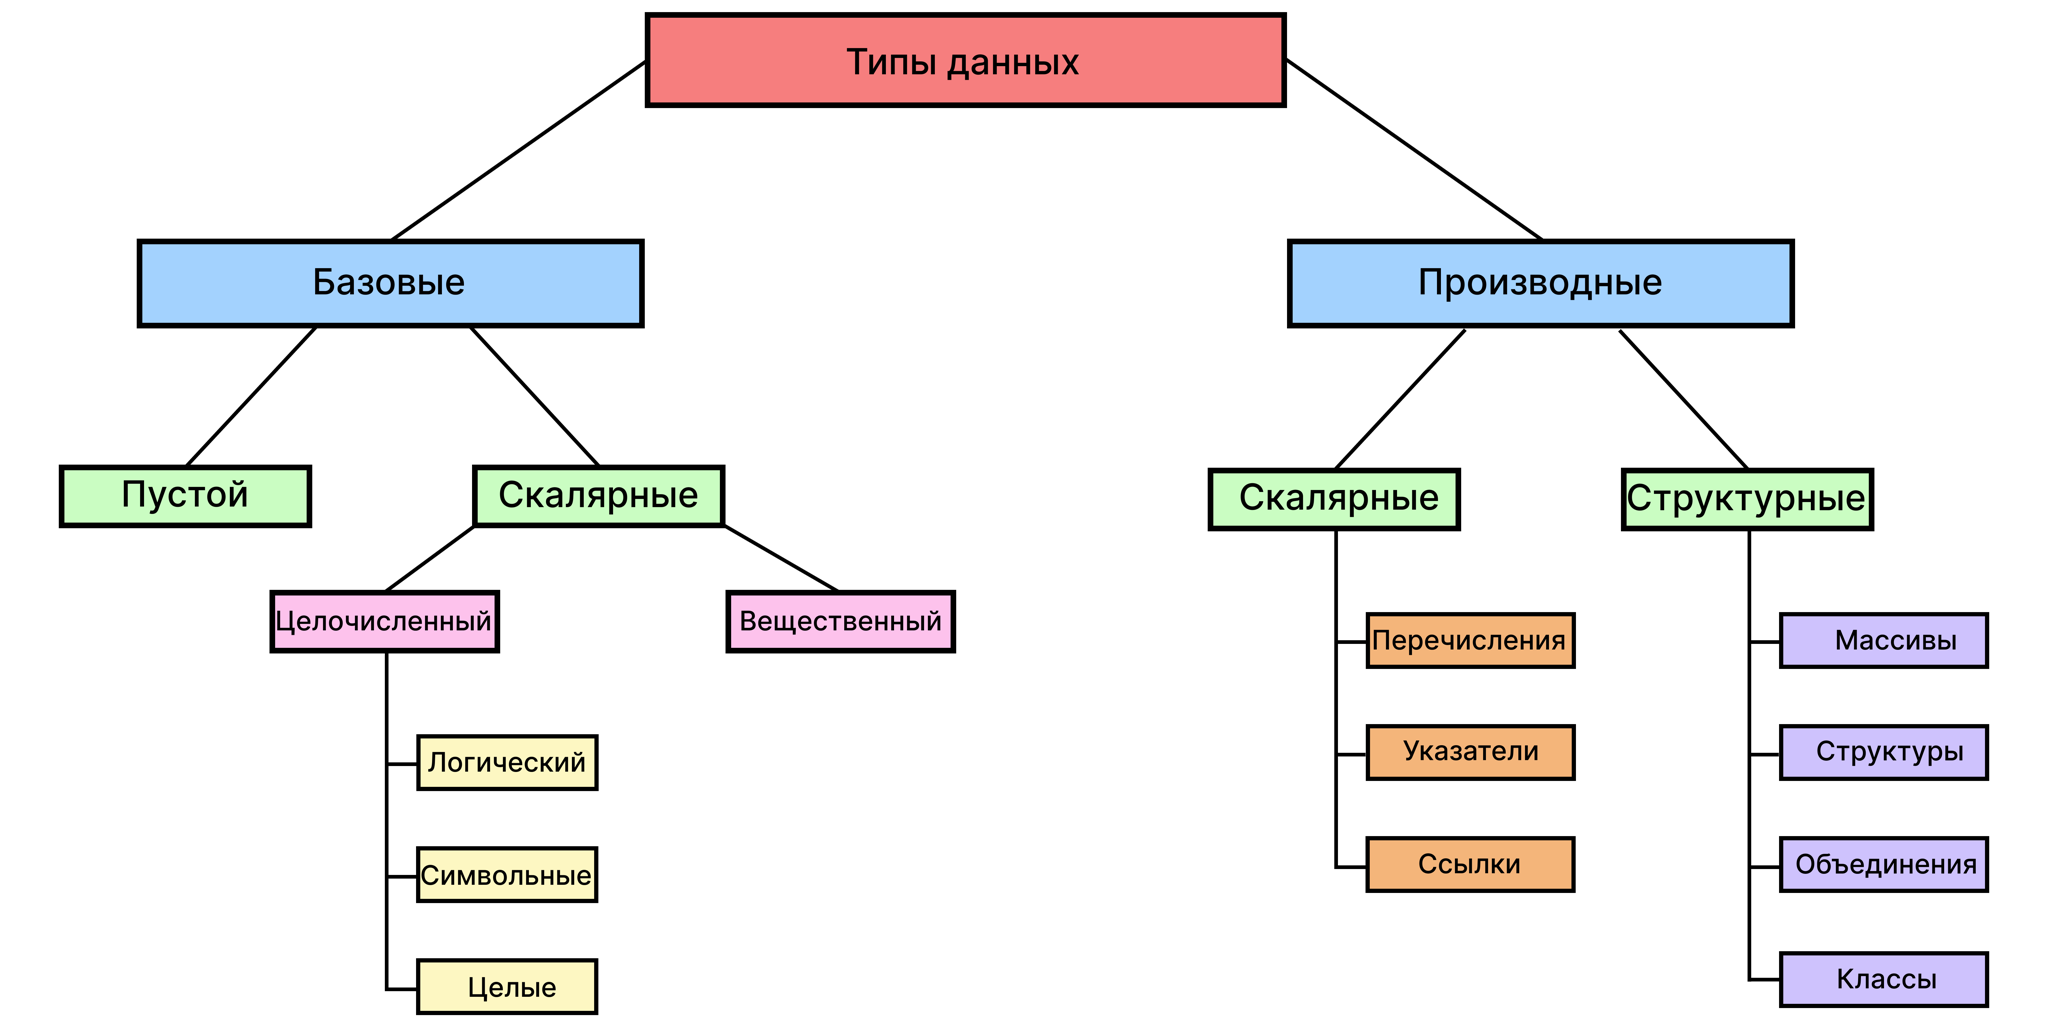
\includegraphics{./res/сpp-types.png}
\caption{Типы данных в C++}
\end{figure}

В категории базовых типов выделяют

\begin{enumerate}
\def\labelenumi{\arabic{enumi})}
\item
  Пустой тип (он же \texttt{void} в \textbf{С++}).

  Нет и не может быть объектов этого типа. Используется в отклонении
  (англ. \emph{discard}) результата вычисления (прим.
  \texttt{(void)GetAnswerToTheUniverse();}) и в функциях, не
  возвращающих значений.
\item
  Скалярные типы

  \begin{itemize}
  \tightlist
  \item
    Целочисленные типы: логический (\texttt{bool} в \textbf{С++}),
    символьный (\texttt{char}, \texttt{wchar\_t}, \texttt{char32\_t},
    \ldots), целый (\texttt{int}, \texttt{short}, \ldots)
  \item
    Вещественный тип
  \end{itemize}
\end{enumerate}

Отдельно рассмотрим целочисленные и вещественные типы данных в
\textbf{С++}.

\subsection{Целочисленные
типы}\label{ux446ux435ux43bux43eux447ux438ux441ux43bux435ux43dux43dux44bux435-ux442ux438ux43fux44b}

Стоит отметить, что размеры конкретных типов зависят от платформы.
Стандарт \textbf{С++} дает ограниченные гарантии на их размер. Также к
ключевым словам типов (\texttt{int}, \texttt{short}, \texttt{long})
могут добавляться квалификаторы \texttt{signed} (определяет знаковость)
и \texttt{unsigned} (определяет беззнаковость). Возможна и комбинация
ключевых слов типов: \texttt{unsigned\ long\ long\ int}.

\begin{longtable}[]{@{}
  >{\raggedright\arraybackslash}p{(\columnwidth - 12\tabcolsep) * \real{0.3418}}
  >{\raggedright\arraybackslash}p{(\columnwidth - 12\tabcolsep) * \real{0.1013}}
  >{\raggedright\arraybackslash}p{(\columnwidth - 12\tabcolsep) * \real{0.1139}}
  >{\raggedright\arraybackslash}p{(\columnwidth - 12\tabcolsep) * \real{0.0759}}
  >{\raggedright\arraybackslash}p{(\columnwidth - 12\tabcolsep) * \real{0.0844}}
  >{\raggedright\arraybackslash}p{(\columnwidth - 12\tabcolsep) * \real{0.1181}}
  >{\raggedright\arraybackslash}p{(\columnwidth - 12\tabcolsep) * \real{0.1646}}@{}}
\toprule\noalign{}
\begin{minipage}[b]{\linewidth}\raggedright
Тип
\end{minipage} & \begin{minipage}[b]{\linewidth}\raggedright
Эквивалентен
\end{minipage} & \begin{minipage}[b]{\linewidth}\raggedright
Пояснение
\end{minipage} & \begin{minipage}[b]{\linewidth}\raggedright
Минимальный размер
\end{minipage} & \begin{minipage}[b]{\linewidth}\raggedright
Размер на \emph{x86-64}
\end{minipage} & \begin{minipage}[b]{\linewidth}\raggedright
Диапазон значений (\emph{x86-64})
\end{minipage} & \begin{minipage}[b]{\linewidth}\raggedright
Примечание
\end{minipage} \\
\midrule\noalign{}
\endhead
\bottomrule\noalign{}
\endlastfoot
\texttt{signed\ char} & \texttt{signed\ char} & Символьный тип & 8 бит &
8 бит & -128 до 127 & \\
\texttt{unsigned\ char} & \texttt{unsigned\ char} & Символьный тип & 8
бит & 8 бит & 0 до 255 & \\
\texttt{char8\_t} & \texttt{char8\_t} & Символьный тип для UTF-8 & 8 бит
& 8 бит & 0 до 255 & С \textbf{С++20} \\
\texttt{wchar\_t} & \texttt{wchar\_t} & Длинный символьный тип & - &
зависит от платформы & зависит от платформы & На Unix/Linux - 32На
Windows - 16 \\
\texttt{char16\_t} & \texttt{char16\_t} & Символьный тип для UTF-16 & 16
бит & 16 бит & 0 до 65535 & \\
\texttt{char32\_t} & \texttt{char32\_t} & Символьный тип для UTF-32 & 32
бит & 32 бит & 0 до 1114111 (\emph{0x10ffff}) & Ограничение Unicode \\
\texttt{short}\texttt{short\ int}\texttt{signed\ short}\texttt{signed\ short\ int}
& \texttt{short\ int} & Целый тип, не больший \texttt{int} & 16 бит & 16
бит & −32768 до 32767 & \\
\texttt{unsigned\ short}\texttt{unsigned\ short\ int} &
\texttt{unsigned\ short\ int} & Беззнаковый \texttt{short} & 16 бит & 16
бит & 0 до 65535 & \\
\texttt{int}\texttt{signed}\texttt{signed\ int} & \texttt{int} &
Основной целый тип & 16 бит & 32 бит & \(-2^{31}\) до \(2^{31}-1\) & \\
\texttt{unsigned}\texttt{unsigned\ int} & \texttt{unsigned\ int} &
Беззнаковый \texttt{int} & 16 бит & 32 бит & 0 до \(2^{32}-1\) & \\
\texttt{long}\texttt{long\ int}\texttt{signed\ long}\texttt{signed\ long\ int}
& \texttt{long\ int} & \emph{Длинное} целое & 32 бит & зависит от
платформы & зависит от платформы & На Unix/Linux - 64Windows API - 32 \\
\texttt{unsigned\ long}\texttt{unsigned\ long\ int} &
\texttt{unsigned\ long\ int} & Беззнаковый \texttt{long} & 32 бит &
зависит от платформы & зависит от платформы & На Unix/Linux - 64Windows
API - 32 \\
\texttt{long\ long}\texttt{long\ long\ int}\texttt{signed\ long\ long}\texttt{signed\ long\ long\ int}
& \texttt{long\ long\ int} & \emph{Дважды длинное} целое & 64 бит & 64
бит & \(-2^{63}\) до \(2^{63}-1\) & \\
\texttt{unsigned\ long\ long}\texttt{unsigned\ long\ long\ int} &
\texttt{unsigned\ long\ long\ int} & Беззнаковый \texttt{long\ long} &
64 бит & 64 бит & 0 до \(2^{64}-1\) & \\
\end{longtable}

\begin{quote}
Тип \texttt{char} занимает по крайней мере 8 бит и ведет себя так же,
как и \texttt{signed\ char} или \texttt{unsigned\ char}, но является
отдельным типом. При этом конкретная знаковость зависит от платформы и
настроек компилятора. На \emph{x86} он обычно знаковый, на \emph{arm} -
обычно беззнаковый.
\end{quote}

\begin{quote}
Логический тип \texttt{bool} занимает по крайней мере 8 бит и хранит
лишь два значения - \texttt{true} или \texttt{false}.
\end{quote}

Типы в \textbf{С++} формируют иерархию по размеру:

\begin{Shaded}
\begin{Highlighting}[]
    \DecValTok{1} \OperatorTok{==} \KeywordTok{sizeof}\OperatorTok{(}\DataTypeTok{char}\OperatorTok{)}\NormalTok{ ≤ }\KeywordTok{sizeof}\OperatorTok{(}\DataTypeTok{short}\OperatorTok{)}\NormalTok{ ≤ }\KeywordTok{sizeof}\OperatorTok{(}\DataTypeTok{int}\OperatorTok{)}\NormalTok{ ≤ }\KeywordTok{sizeof}\OperatorTok{(}\DataTypeTok{long}\OperatorTok{)}\NormalTok{ ≤ }\KeywordTok{sizeof}\OperatorTok{(}\DataTypeTok{long} \DataTypeTok{long}\OperatorTok{)}
\end{Highlighting}
\end{Shaded}

Однако стандарт гарантирует лишь минимальное количество бит типов. В
частности возможная абсурдная ситуация, когда на платформе один байт*
занимает 64 бит и

\begin{Shaded}
\begin{Highlighting}[]
    \KeywordTok{sizeof}\OperatorTok{(}\DataTypeTok{char}\OperatorTok{)} \OperatorTok{==} \KeywordTok{sizeof}\OperatorTok{(}\DataTypeTok{short}\OperatorTok{)} \OperatorTok{==} \KeywordTok{sizeof}\OperatorTok{(}\DataTypeTok{int}\OperatorTok{)} \OperatorTok{==} \KeywordTok{sizeof}\OperatorTok{(}\DataTypeTok{long}\OperatorTok{)} \OperatorTok{==} \KeywordTok{sizeof}\OperatorTok{(}\DataTypeTok{long} \DataTypeTok{long}\OperatorTok{)} \OperatorTok{==} \DecValTok{1}
\end{Highlighting}
\end{Shaded}

Количество бит, которое занимает тип \texttt{char} можно проверить
макросом \texttt{CHAR\_BIT}; впрочем, практически все современные
системы имеют байт* равным 8 бит.

*под байтом в этом контексте понимается минимально адресуемый объем
памяти. Это не обязательно `байт' в значении объем информации.

\subsection{Вещественные
типы}\label{ux432ux435ux449ux435ux441ux442ux432ux435ux43dux43dux44bux435-ux442ux438ux43fux44b}

Стандарт \textbf{С++} определяет следующие типы с плавающей точкой: 1)
\texttt{float} - вещественный тип одинарной точности. Обычно
\textbf{IEEE 754} \emph{binary32}. 2) \texttt{double} - вещественный тип
двойной точности. Обычно \textbf{IEEE 754} \emph{binary64}. 3)
\texttt{long\ double} - вещественный тип повышенной точности.

\begin{verbatim}
На разных платформах может быть типом четверной точности (**IEEE 754** *binary128*), 80-битным *x87-80 extended precision format* на *x86*, быть эквивалентным `double` или реализован каким-либо другим образом.
\end{verbatim}

% \section{Представление данных в оперативной памяти. Хранение переменных в Стеке}

\subsection{Представление данных в памяти}

\textbf{Бит} --- это самая маленькая единица измерения информации. Биты
складываются в байты, те --- в килобайты, мегабайты и так далее.
Название произошло от слов binary digit, двоичное число. Это значит, что
в одном бите может храниться одно из двух значений: 0 или 1.

\textbf{Байт} --- единица хранения и обработки цифровой информации;
совокупность битов, обрабатываемая компьютером одновременно.

Под \textbf{адресом} будем понимать номер начального байта.

Различные данные представляются в оперативной памяти компьютера
различным образом.

\subsubsection{Целые числа}

Беззнаковые целые числа просто хранятся в памяти компьютера в двоичном
коде. Однако знаковые числа требуют хранения особым образом, для
однозначного разделения отрицательных и положительных чисел. Существуют
3 стандартных способа хранения отрицательных чисел: прямой код, обратный
код и дополнительный код.

\begin{enumerate}
\def\labelenumi{\arabic{enumi})}
\item
  Прямой код (англ. \emph{sign and magnitude}).

  Старший бит двоичной записи числа называется знаковым битом. Если он
  установлен, число считается отрицательным, иначе положительным. Имеет
  проблему 2 нулей (\(10000000_2=00000000_2=0_{10}\)) и невозможности
  напрямую проводить арифметические операции
  (\(5_{10}(00000101_2) + -5_{10}(10000101_2) = 10001010_2 \ne 0_{10}\)).
\item
  Обратный код (англ. \emph{one's complement}).

  Отрицательные числа кодируются как побитовая инверсия противоположных
  положительных чисел. Имеет проблему 2 нулей
  (\(00000000_2=11111111_2=0_{10}\)).
\item
  Дополнительный код (англ. \emph{two's complement})

  Отрицательные числа кодируются как побитовая инверсия положительных
  чисел плюс число 1. Не имеет названных проблем (только 1 ноль,
  арифметика стандартна).
\end{enumerate}

Начиная с \textbf{С++20} единственной разрешенной формой кодирования
знаковых отрицательных чисел в С++ является \textbf{дополнительный код}.

\subsubsection{Вещественные числа}

Стандарт не регламентирует строго формат хранения вещественных чисел,
однако на фактически всех современных пользовательских и серверных
платформах они представлены числами \textbf{IEEE 754}.

\textbf{IEEE 754} регламентирует
\begin{enumerate}
  \item Двоичное представление чисел с плавающей запятой;
  \item Допустимые операции над такими числами;
  \item Их поведение при выполнении операций, в частности, методы округления;
  \item Специальные значения (\emph{NaN}, \emph{infinity}).
\end{enumerate}

В общем виде числа \textbf{IEEE 754} хранятся в памяти в следующем виде
(на примере binary32, float в \textbf{С++}):

\begin{figure}
\centering
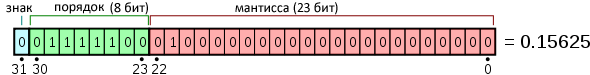
\includegraphics{./res/ieee-binary32.png}
\caption{IEEE-754 binary32}
\end{figure}

А представляются в виде 
\begin{enumerate}
   \item \((-1)^s \times 1.M \times 2^E\), если \(E_{min} \le E \le E_{max}\) (нормализованные числа),
   \item \((-1)^s \times 0.M \times 2^{E_{min}}\), если \(E=E_{min}-1\) (денормализованные числа),
\end{enumerate}
где - s - знак - M - мантисса - E - порядок (англ. exponent)

\subsection{Стек. Хранение локальных переменных}

\textbf{Стек} - особая область памяти, работающая по принципу ``первый
зашел, последний вышел'' (\textbf{FILO}), хранящая информацию о текущей
подпрограмме и возврате из подпрограммы в вызвавшую программу
(подпрограмму).

Структура, выравнивание, размер и положение стека в памяти определяется
платформой; порядок вызова функций и хранение локальных переменных также
определяется платформой. Обычно эти параметры определяются
\textbf{двоичным интерфейсом приложения} (англ. \textbf{ABI} -
\textbf{application binary interface}) платформы, а его часть касательно
порядка вызова функций - \textbf{соглашением о вызовах} (англ.
\emph{calling convention}).

Например, на \emph{x86-64} стек растет от старших адресов к младшим:

\begin{figure}
\centering
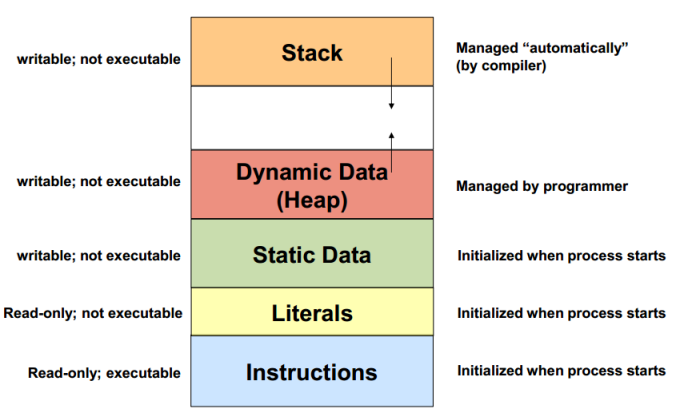
\includegraphics{./res/mem.png}
\caption{Секции памяти в С++}
\end{figure}

Аргументы и локальные переменные функций также в общем случае хранятся
на стеке. При входе в функцию на стеке под нее выделяется \emph{кадр
стека} - там хранятся переменные и аргументы, а также адрес возврата из
функции. При выходе из функции кадр стека уничтожается (точнее, вершина
стека перемещается вверх, за этот кадр, поэтому содержимое становится
недоступным). Очистка памяти на стеке происходит автоматически, без
участия программиста.

% \section{Представление алгоритмов. Блок-схемы}

\textbf{Алгоритм} -- это точное предписание, определяющее вычислительный
процесс, ведущий от варьируемых начальных данных к искомому результату.

Алгоритм может быть представлен различным образом: 1) Словесный;

\begin{verbatim}
Предполагает описание алгоритма на естественном языке. Имеет существенный недостаток - строго не формализуем.
\end{verbatim}

\begin{enumerate}
\item
  Формульно-словесный;

  Алгоритм записывается в виде текста с формулами по пунктам,
  определяющим последовательность действий.
\item
  \textbf{Блок-схемный};
\item
  Псевдокод;

  \emph{Псевдокод} - компактный, зачастую неформальный язык описания
  алгоритмов, использующий ключевые слова императивных языков
  программирования, но опускающий несущественные для понимания алгоритма
  подробности и специфический синтаксис.
\item
  Структурные диаграммы;

  \emph{Структурные диаграммы} описывают структуру сложных объектов и
  систем, показывают статическую структуру системы и ее частей на разных
  уровнях абстракции и реализации, а также их взаимосвязь.
\item
  Языки программирования

  \emph{Алгоритмический язык} --- это искусственный язык (система
  обозначений), предназначенный для записи алгоритмов. Он позволяет
  представить алгоритм в виде текста, составленного по определенным
  правилам с использованием специальных служебных слов. Количество таких
  слов ограничено. Каждое служебное слово имеет точно определенный
  смысл, назначение и способ применения.

  \textbf{Язык программирования} - алгоритмический язык, команды
  которого однозначно преобразуются в команды для компьютера.
\end{enumerate}

\subsection{Блок-схемы}\label{ux431ux43bux43eux43a-ux441ux445ux435ux43cux44b}

\textbf{Блок--схема} --- наглядный способ представления алгоритма.
Блок--схема отображается в виде последовательности связанных между собой
\emph{функциональных блоков}, каждый из которых соответствует выполнению
одного или нескольких действий. Определенному типу действия
соответствует \emph{определенная геометрическая фигура блока}. Линии,
соединяющие блоки, определяют \emph{очередность выполнения действий}. По
умолчанию блоки соединяются \emph{сверху вниз и слева направо}. Если
последовательность выполнения блоков должна быть иной, используются
направленные линии (стрелки).

Блок-схемы регламентируются такими документами, как \textbf{ГОСТ
19.701-90}, \textbf{СТП 01-2017} (стандарт предприятия БГУИР).

\begin{figure}
\centering
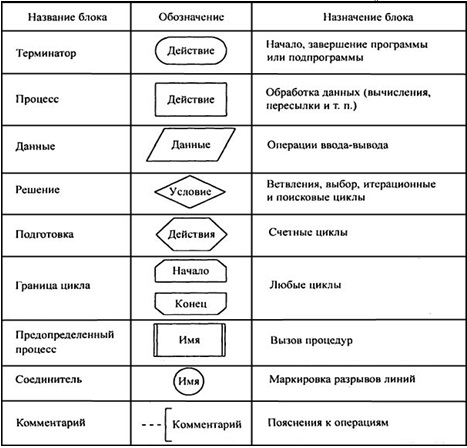
\includegraphics{./res/schematics.png}
\caption{Обозначения на блок-схемах}
\end{figure}

Пример блок-схемы алгоритма:

% \section{Выражения: математические, логические,
текстовые}\label{ux432ux44bux440ux430ux436ux435ux43dux438ux44f-ux43cux430ux442ux435ux43cux430ux442ux438ux447ux435ux441ux43aux438ux435-ux43bux43eux433ux438ux447ux435ux441ux43aux438ux435-ux442ux435ux43aux441ux442ux43eux432ux44bux435}

\textbf{Операнд} - объект над которым происходит операция.

\textbf{Выражение} - комбинация знаков операций и операндов, результатом
которой является определенное значение. Знаки операций определяют
действия, которые должны быть выполнены над операндами. Каждый операнд в
выражении может быть выражением. Значение выражения зависит от
расположения знаков операций и круглых скобок в выражении, а также от
приоритета выполнения операций.

Каждое выражение в С++ характеризуется своим типом. Результирующий тип
выражения выводится из типов операндов и характера операций.

При вычислении выражений тип каждого операнда может быть преобразован к
другому типу. Преобразования типов могут быть неявными, при выполнении
операций и вызовах функций, или явными, при выполнении операций
приведения типов.

\subsection{Логические
выражения}\label{ux43bux43eux433ux438ux447ux435ux441ux43aux438ux435-ux432ux44bux440ux430ux436ux435ux43dux438ux44f}

Результатом логического выражения есть объект логического типа - истина
или ложь. Такие выражения соотносятся с выражениями из булевой алгебры и
используются в первую очередь в операторах ветвления и цикла.

\subsection{Текстовые выражения\footnote{Текстовых выражений в С++ нет. По крайней мере, никакой информации на этот счет найдено не было.}}
Строковые литералы в C++ имеют тип указателя на массив символьного типа:
\begin{minted}{C++}
const char *normal_str = "A normal string";
const char8_t *utf8_str = u8"A UTF-8 string";
const char16_t *utf16_str = u"A UTF-16 string";
const char32_t *utf32_str = U"A UTF-32 string";

const wchar_t *long_string = L"A long (wide) string";
\end{minted}

\subsection{Математические
выражения}\label{ux43cux430ux442ux435ux43cux430ux442ux438ux447ux435ux441ux43aux438ux435-ux432ux44bux440ux430ux436ux435ux43dux438ux44f}

\textbf{Математическое выражение} - это совокупность знаков, описывающая
отношение между какими-то величинами. Результатом математических
выражений обычно является какое-либо число.

В С++ поддерживается арифметика целых и вещественных чисел, а также указателей
(кроме \minline{void*} и указателей на функции).
% \section{Унарные
операции}\label{ux443ux43dux430ux440ux43dux44bux435-ux43eux43fux435ux440ux430ux446ux438ux438}

\textbf{Унарная операция} - операция над одним операндом и возвращающая
один результат.

Рассмотрим унарные операции в \textbf{С++}.

\begin{enumerate}
\def\labelenumi{\arabic{enumi})}
\item
  Унарные `плюс' и `минус'
\begin{minted}{C++}
  +a;
  -a;
\end{minted}

  Унарный плюс не изменяет выражения, унарный минус меняет знак на
  противоположный.
\item
  Префиксный/постфиксный инкремент и декремент
\begin{minted}{C++}
  ++a;
  a++;
  --a;
  a--;
\end{minted}

  Прибавляет (инкремент) или отнимает (декремент) \(1\). Меняет операнд.
  В префиксной форме, сначала прибавляет/отнимает, потом возвращает
  значение измененной переменной. В постфиксной, сначала возвращает
  исходное значение переменной, потом прибавляет/отнимает.
\item
  Отрицание (логическое НЕ)
\begin{minted}{C++}
  !a;
\end{minted}

  Заменяет \texttt{true} на \texttt{false}, а \texttt{false} - на
  \texttt{true} и возвращает \textbf{логическое значение} - результат
  такой замены. Сам операнд не изменяется.
\item
  Побитовая инверсия
\begin{minted}{C++}
  ~a;
\end{minted}

  Заменяет \(0\) в двоичной записи числа на \(1\), а \(1\) - на \(0\) и
  возвращает \textbf{число} - результат такой замены. Сам операнд не
  изменяется.
\item
  Взятие адреса и косвенная адресация
\begin{minted}{C++}
  int *address = &a;
  *a = 42;
\end{minted}

  Взятие адреса применяется к переменной и возвращает адрес первой
  ячейки памяти, где хранится эта переменная, в виде указателя.
  Косвенная адресация позволяет прочитать и записать по адресу,
  хранящемуся в указателе.
\item
  Оператор \texttt{sizeof()} - получение размера типа
\begin{minted}{C++}
  sizeof(a)
\end{minted}
  Возвращает размер типа(типа выражения) в байтах. Стандарт допускает,
  что байт может не быть равен 8 бит, поэтому точнее говорить, что
  \texttt{sizeof} возвращает размер типа в адресуемых ячейках памяти.
\end{enumerate}

\begin{enumerate}
\def\labelenumi{\arabic{enumi})}
\setcounter{enumi}{6}
\item
  Оператор приведения типов в стиле С
\begin{minted}{C++}
    int a = 42;
    double c_style = (double)a;
\end{minted}
\item
  выделение и освобождение памяти - \texttt{new} и \texttt{delete}
\begin{minted}{C++}
  int *heap_allocated = new int;
    *heap_allocated = 42;

    //...

    delete heap_allocated;
\end{minted}
\end{enumerate}

\ldots и хватит\ldots{}

% \section{Классификация бинарных операций}

\textbf{Бинарная операция} - операция над двумя операндами и
возвращающая один результат.

К бинарным операциям в С++ относятся:

\begin{enumerate}
\def\labelenumi{\arabic{enumi})}
\item
  Присваивания
  (\texttt{=\ +=\ -=\ *=\ /=\ \%=\ \&=\ \textbar{}=\ \^{}=\ \textgreater{}\textgreater{}=\ \textless{}\textless{}=});
\item
  Арифметические, за исключением унарных \texttt{+}, \texttt{-}
  (\texttt{+\ -\ *\ /\ \%});
\item
  Побитовые, за исключением побитовой инверсии
  \texttt{\textasciitilde{}}
  (\texttt{\&\ \textbar{}\ \^{}\ \textless{}\textless{}\ \textgreater{}\textgreater{}});
\item
  Логические, за исключением унарного логического отрицания \texttt{!}
  (\texttt{\&\&\ \textbar{}\textbar{}});
\item
  Сравнения
  (\texttt{==\ !=\ \textless{}\ \textgreater{}\ \textless{}=\ \textgreater{}=\ \textless{}=\textgreater{}});
\item
  Обращения к члену ( \texttt{-\textgreater{}\ .});
\item
  Другие особые операторы:

  \begin{itemize}
  \item
    Оператор разрешения области видимости (\texttt{::})
  \item
    Оператор \texttt{,} (запятая)
  \item
    Встроенный (неперегруженный) оператор \texttt{{[}{]}} (в С++23 этот
    оператор может иметь любую -арность, как и оператор вызова функции,
    но только в перегруженном виде. Встроенный оператор
    \texttt{E1{[}E2{]}} эквивалентен \texttt{*(E1\ +\ E2)})
  \end{itemize}
\end{enumerate}

% \section{Арифметические и поразрядные операции. Результат операции}

Пусть \texttt{a}, \texttt{b} - операнды. К арифметическим операциям в
С++ относятся:

\begin{longtable}[]{@{}lll@{}}
\toprule\noalign{}
Операция & Вызов & Тип операндов \\
\midrule\noalign{}
\endhead
\bottomrule\noalign{}
\endlastfoot
Сложение & \texttt{a\ +\ b} & Целые/вещественные числа \\
Вычитание & \texttt{a\ -\ b} & Целые/вещественные числа \\
Умножение & \texttt{a\ *\ b} & Целые/вещественные числа \\
Деление нацело & \texttt{a\ /\ b} & Целые числа \\
Вещественное деление & \texttt{a\ /\ b} & Вещественные числа \\
Взятие остатка от деления & \texttt{a\ \%\ b} & Целые числа \\
Унарный плюс & \texttt{+a} & Целое/вещественное число \\
Унарный минус & \texttt{-a} & Целое/вещественное число \\
\end{longtable}

Результатом арифметических операций являются числа (целые или
вещественные).

Пусть n - число разрядов (бит) в числах \texttt{a} и \texttt{b}. Пусть
также \(a[i]\) означает \(i\)-ый бит числа a. К поразрядным операциям в
С++ относятся:

\begin{longtable}[]{@{}
  >{\raggedright\arraybackslash}p{(\columnwidth - 6\tabcolsep) * \real{0.3223}}
  >{\raggedright\arraybackslash}p{(\columnwidth - 6\tabcolsep) * \real{0.0795}}
  >{\raggedright\arraybackslash}p{(\columnwidth - 6\tabcolsep) * \real{0.1280}}
  >{\raggedright\arraybackslash}p{(\columnwidth - 6\tabcolsep) * \real{0.5303}}@{}}
\toprule\noalign{}
\begin{minipage}[b]{\linewidth}\raggedright
Операция
\end{minipage} & \begin{minipage}[b]{\linewidth}\raggedright
Вызов
\end{minipage} & \begin{minipage}[b]{\linewidth}\raggedright
Тип операндов
\end{minipage} & \begin{minipage}[b]{\linewidth}\raggedright
Примечание
\end{minipage} \\
\midrule\noalign{}
\endhead
\bottomrule\noalign{}
\endlastfoot
Побитовое И & \texttt{a\ \&\ b} & Целые числа & \texttt{r\ =\ a\ \&\ b;}
\(\forall i=1...n,\ r[i] = a[i] \land b[i]\) \\
Побитовое ИЛИ & \texttt{a\ \textbar{}\ b} & Целые числа
& \texttt{r\ =\ a\ \textbar{}\ b;}
\(\forall i=1...n,\ r[i] = a[i] \lor b[i]\) \\
Побитовое ИСКЛЮЧАЮЩЕЕ ИЛИ & \texttt{a\ \^{}\ b} & Целые числа &
\texttt{r\ =\ a\ \^{}\ b;}
\(\forall i=1...n,\ r[i] = a[i] \oplus b[i]\) \\
Побитовая инверсия & \texttt{\textasciitilde{}a} & Целое число &
\texttt{r\ =\ \textasciitilde{}a;}
\(\forall i=1...n,\ r[i] = \neg{a[i]}\) \\
Побитовое сдвиг вправо & \texttt{a\ \textless{}\textless{}\ b} & Целые
числа & Сдвигает биты числа \texttt{a} на \texttt{b} разрядов влево.
Если \(b > n\) или \(b < 0\), результат не определен \\
Побитовый сдвиг влево & \texttt{a\ \textgreater{}\textgreater{}\ b} &
Целые числа & Сдвигает биты числа \texttt{a} на \texttt{b} разрядов
вправо. Если \(b > n\) или \(b < 0\), результат не определен.Результат
также не определен, если \(a < 0\), хотя большинство платформ применят
расширение знаковым битом \\
\end{longtable}

Результатом поразрядных операций являются целые числа.


\addcontentsline{toc}{section}{Вопросы 19-36}
\phantomsection
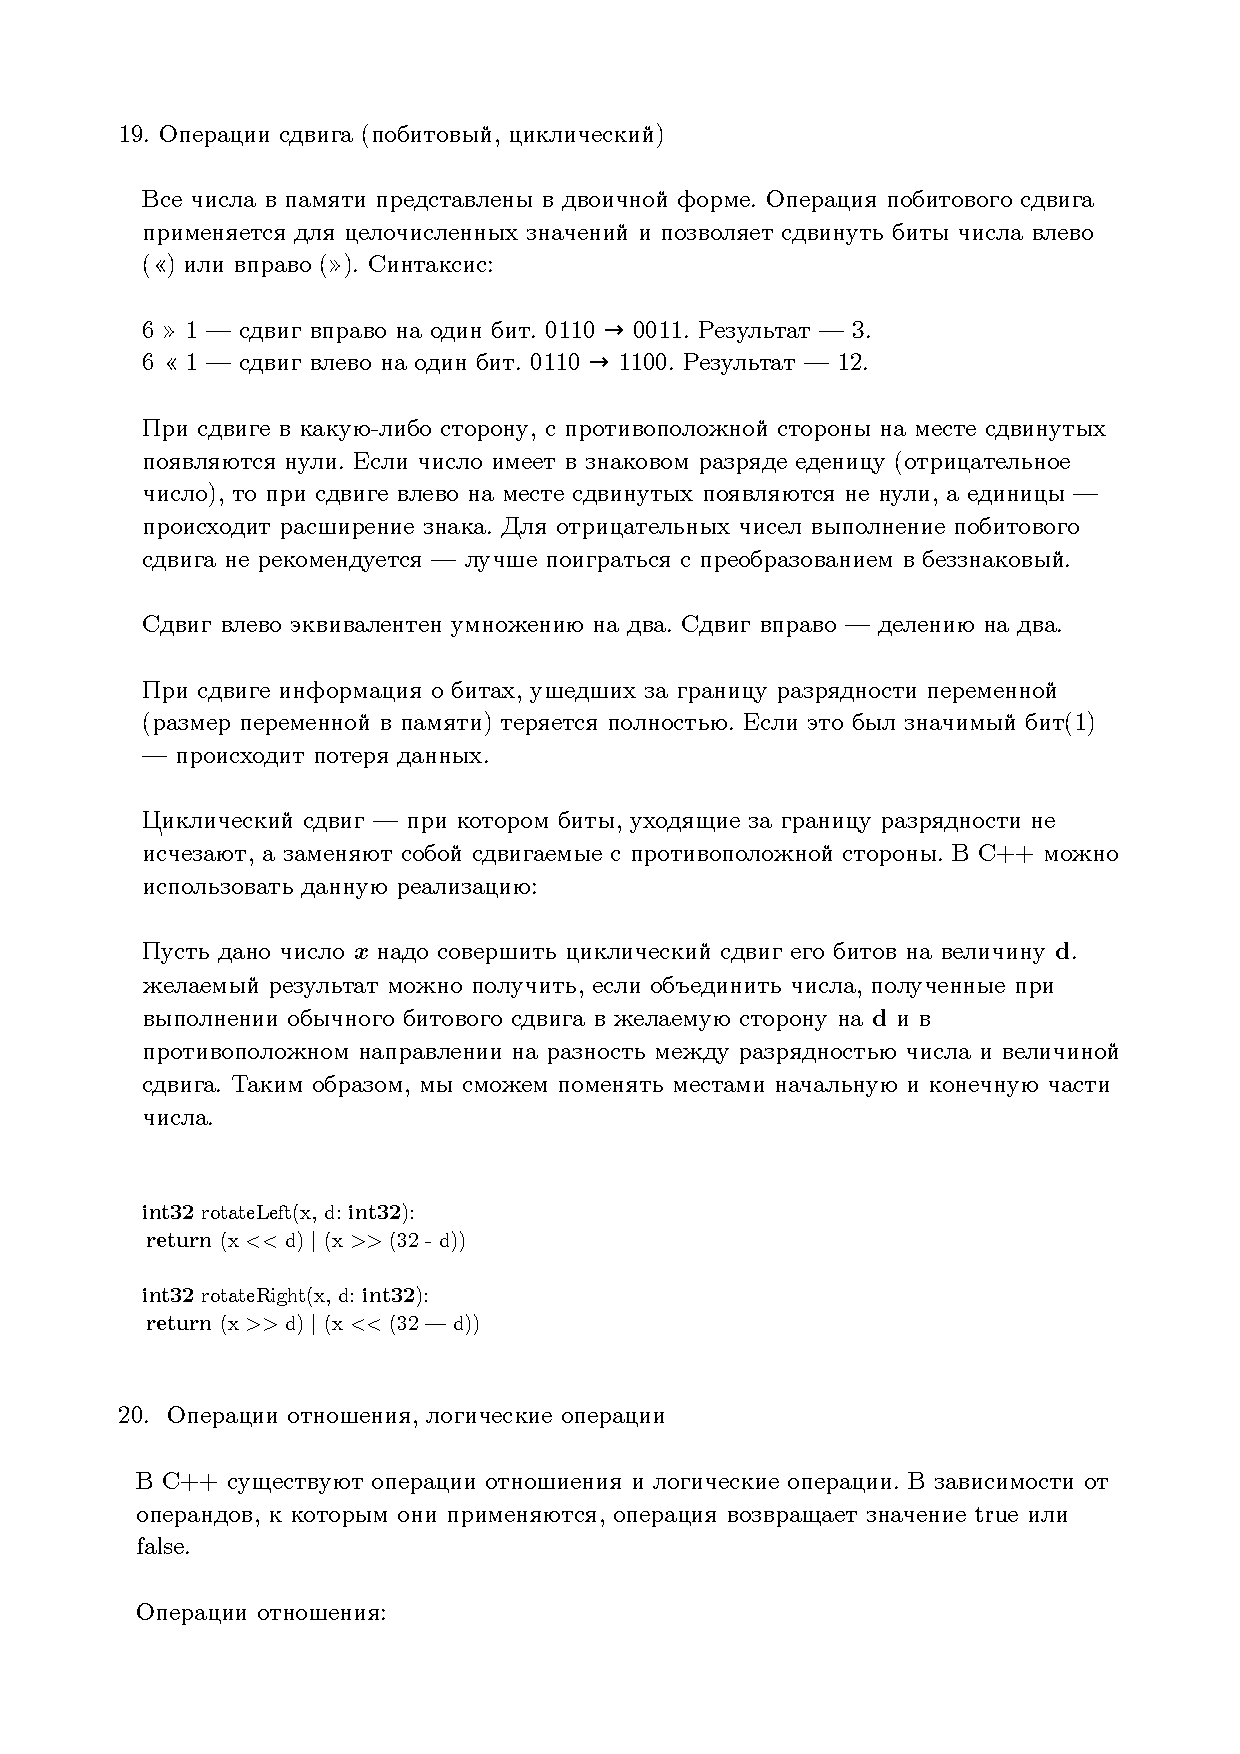
\includepdf[pages=-]{19-36.pdf}

\setcounter{section}{36}
\section{Операции над указателями разного порядка}
Над указателями можно проводить следующие операции:
\begin{enumerate}
  \item Присваивание \verb|=|. Работает так же, как и с обычными переменными:
  операция \verb|a = b| запишет в указатель \verb|a| значение указателя \verb|b|
  и вернет записанное значение. Присваивание разрешено только если оба операнда одноименные
  или один из них является указателем на \verb|void|. С данными, на которые указывал \verb|a|,
  ничего не будет. Если на эти данные не было других указателей, то доступ к ним будет
  утерян и освобождения памяти не последует.
  \item Разыменование \verb|*| возвращает тот объект, на который указывает указатель.
  \begin{verbatim}
int *a = 4;
// 4
std::cout << a << '\n';
*a += 7;
// 11
std::cout << *a << '\n';
  \end{verbatim}
  \item Взятие адреса самой перменной, которая является указателем \verb|&| возвращает указатель
  на указатель (то есть указатель высшего порядка):
  \begin{verbatim}
int a = 13;
int *b = &a;
int **c = &b;
int ***d = &c;
// ...
// Можно продолжать сколько угодно

// 13
std::cout << **c << '\n';
// Два одинаковых числа
std::cout << *d << ' ' <<c << '\n';
  \end{verbatim}
  \item Сравнение значений указателей \verb|<, <=, >, >=, ==, !=|. Адреса, на которые
  указыввают сравниваемые указатели сравниваются как обычные целые числа.
  \item \hyperref[sec:ptr_arithm]{Арифметические операции}.
\end{enumerate}

Все эти операции работают для указателей любого порядка.

Указатели высших порядков обычно используются в для представления многомерных
массивов\footnote{адекватные люди (если они программируют не микроконтроллеры)
для этого используют вложенные \mbox{std::vector}}.
Для получения конкретного элмента $n$-мерного массива достаточно $n$ раз
применить оператор \verb|[]|\footnote|или сложения с разыменованиями, если вы желаете страдать|.

Перебор многомерных массивов осуществляется с помощбю вложенных циклов
Ниже приведен пример сложения матриц.

\begin{verbatim}
/// Складывает матрицы `lhs` и `rhs` размера `m * n`.
/// Результат записывает в матрицу `res`.
void AddMatrices(int **lhs, int **rhs, int **res,
                 int m, int n)
{
  for (int i = 0; i < m; ++m) {
    for (int j = 0; j < n; ++j) {
      // Вместо того, что в левой части
      // для доступа к элементам массива `res`
      // можно использовать выражение `res[i][j]`
      *(*(res + i) + j) = lhs[i][j] + rhs[i][j];
    }
  }
}
\end{verbatim}

\section{Арифметика указателей}
\label{sec:ptr_arithm}
\textbf{Указатель} --- переменная, значением которой является адрес памяти.
В памяти указатель представляется как беззнаковое целое длины, равной длине
машинного слова.
\textit{Одноименными} будем называть указатели, которые указывают на переменные
одинакового типа. По стандарту арифметические операции нельзя совершать над 
указателями на \verb|void|\footnote{точнее, на неполные типы (incomplete types ---
types that describe objects but lack information needed to determine their sizes)}
и функции, хотя GCC разрешает эти операции в качестве расширения.

К арифметическим операциям над указательями относятся следующие операции:
\begin{enumerate}
  \itembf{Сложение с числом.} К указателю можно прибавлять как положительные,
  так и отрицательные числа. Эта операция коммутативна. При прибавлении к указателю
  \verb|a| числа \verb|n|, значение адреса памяти, на котороый указвает указатель,
  увеличивается на \verb|n*sizeof(*a)|. Таким образом, указатель сдвигается на одну или
  несколько ячеек.

  Выражение \verb|*(a + n)| также можно записывать как \verb|a[n]|.
  С точки зрения языка обе записи эквивалентны.
  Пример (выведет \verb|OK|):
\begin{verbatim}
int n = 4;
if (((unsigned long) (a+n)) ==
    ((unsigned long) a) + (n*sizeof(int))) {
      std::cout << "OK\n";
}
\end{verbatim}

  \itembf{Инкремент и декремент} прибавляет и отнимает единицу к указателю (\textbf{не} к адресу!) по правилу, указанному
  выше, соответственно. При этом, как и с обычными чисами, префиксные операторы возвращают измененное
  значение, а постфиксные --- неизмененное.

  Единственное, следует обратить внимание на приоритет оператора инекремента (декремента)
  и оператора разыменования \verb|*|. При использовании как префиксного, так и постфиксного
  оператора сначала выполнится инкремент (декремент) и только потом --- разыменование.
\begin{verbatim}
int c[2]{5, 10};
int *b = c;
// 5 (b до изменения указывает на c[0])
std::cout << *b++ << '\n';
// Теперь b указывает на c[1]
// 10 | 5 10
std::cout << *b << " | " << c[0] << ' '
                          << c[1] << '\n';
\end{verbatim}

  \itembf{Вычитание числа из указателя} работает так же, как и прибавление к указателю
  числа, противоположного по знаку.
  \itembf{Вычитание одноименных указателей} \verb|a - b| возвращает такое число \verb|n|,
  что \verb|a == b + n|. Число \verb|n| имеет тип \verb|ptrdiff_t| из \verb|<cstddef>|,
  который является \verb|typedef|'ом от какого-то\footnote{implementation-defined} базового
  \textit{знакового} целочисленного типа.
\begin{verbatim}
int a[20]{};
int *b = a;
int *c = a + 12;
// 12
std::cout << c - b << '\n';
// -12
std::cout << b - c << '\n';
\end{verbatim}
  Если результат вычитания настолько большой, что не может поместиться в \verb|ptrdiff_t|,
  то UB.
\end{enumerate}

\section{Массивы переменных размеров. Аллокаторы памяти}
\textbf{Массив} — это определённое число ячеек памяти, расположенных непосредственно друг за другом.
Массив позволяет хранить несколько значений одинакового типа.

Поскольку число элементов массива переменной длины и, следовательно, его размер заранее неизвестны,
память для него обычно выделяется в куче. Доступ к элементам массива при этом осуществляется через
указатель на первый элемент массива при помощи арифметики указателей или оператора \verb|[]|

В языке C++ память можно выделять двумя основными способами:
\begin{enumerate}
  \item Функциии \verb|malloc, realloc, calloc|.
  Для первоначального выделения памяти можно использовать любую из этих функций.
  Для изменения размера выделенного участка памяти необходимо использовать 
  функцию \verb|realloc|. Она либо расширяет старый участок памяти, либо выделяет память
  заново, копирую при этом туда нужное число элементов (минимум от старого и нового размеров) и
  освобждая после этого старый участок.

  \begin{verbatim}
// Выделение памяти
int *array = (int*) malloc(sizeof(int) * array_size);

// Изменение размера
array = (int*) realloc(sizeof(int) * new_array_size);

// Освобождение памяти
free(array);
  \end{verbatim}
  
  \item Оператор \verb|new[]|
  Оператор \verb|new type[x]| позволяет выделети динамический массив из \verb|x|
  элементов типа \verb|type|, вызывая для каждого элемента конструктор по умолчанию.
  Для освобождения выделенного массива используется операвтор \verb|delete[]|, который
  не только освободит память, но и вызовет деструкторы всех элементов массива.

  Язык C++ не предоставляет аналога функции \verb|realloc| из C. Поэтому для изменения размера массива
  необходимо выделить память заново и вручную переместить
  в новую область памяти существующие элементы массива.
  \begin{verbatim}
// Выделение памяти
int *array = new int[array_size];

// Изменение размера
int *new_array = new int[new_array_size];
int copy_size = std::min(array_size, new_array_size);
for (int i = 0; i < copy_size; ++i) {
  new_array[i] = array[i]; // Или std::move(array[i]);
}
delete[] array;
array = new_array;

// Освобождение памяти
delete[] array;
  \end{verbatim}
\end{enumerate}

Работа с памятью в стиле языка Си в некоторых случаях позволяет облегчить
перевыделение памяти, поскольку избегает копирования всех элементов массива,
однако возлагает на программиста ответственность за ручной вызов деструкторов
и placement new, если приходится работать с объектами производных типов.

\paragraph{Аллокатор} --- высокоуровневая абстракция над выделением и освобождением памяти,
которая позволяет задать конекретный способ того, как будет выделяться память. Аллокатор
должен предоставлять функционал выделения и освобождения выделенной им памяти.

Для непосредственного выделения памяти используются системные вызовы
\verb|mmap| на Linux; \verb|GlobalAlloc|, \verb|HeapAlloc| и др. на Windows.
Они требуют переключения контекста на процессоре и передают управление ядру ОС,
что является относительно дорогостоящей операцией. Из-за этого программисты обычно
стремятся уменьшить число системных вызовов.

В случае выделения памяти этого можно достичь, если, например, обращаться к системным вызовам
только для выделения достаточно больших участков памяти, которые распределяются уже функциями,
которые работают в пространстве пользователя.

Примерно такую стратегию используют функции \verb|*alloc| и оператор \verb|new|, поэтому
в широком смысле их можно назвать аллокаторами.

Наконец, отметим, что аллокатор в общем случае не обязан выделять память на куче или вообще использовать
системные вызовы. Ниже приведен пример примитивного аллокатора, который выделяет статическую память.

Он резервирует 100\,000 байт статической памяти и хранит размер
выделенной памяти, а вызове метода \verb|Allocate| возвращает указатель на участок
зарезрвированной при создании памяти и увеличивает значение переменной, хранящей
размер выделенной памяти.

Для простоты реализации этот аллокатор не может переиспользовать освобожденную память,
поэтому функция \verb|Deallocate|, которая должна освобождать участок памяти, ничего не
делает. Вся память, занятая аллокатором будет атоматически осовобождена при завершении исполнения прграммы.

\begin{verbatim}
#include <cmath>
#include <iostream>

struct StaticAllocator {
  static constexpr const size_t kPoolSize = 100'000;

  /// Выделяет память размером `size`'.
  /// В случае неудачи возвращает `nullptr`,
  /// иначе - указатель на выделенную память.
  void *Allocate(size_t size) {
    if (allocated_ + size <= kPoolSize) {
      void *result = pool_ + allocated_;
      allocated_ += size;
      return result;
    }
    return nullptr;
  }
  /// Освобождает выделенный указатель `ptr`
  void Deallocate(void *ptr) {
    /// nop
  }

private:
  char pool_[kPoolSize];
  size_t allocated_ = 0;
};

static StaticAllocator allocator;

int main() {
  // Массив из 3 int'ов
  int *a = (int *)allocator.Allocate(3 * sizeof(int));
  std::cin >> a[0];
  std::cin >> a[1];
  a[2] = a[0] + a[1];
  std::cout << a[2] << '\n';

  // Один double
  double *b = (double *)allocator.Allocate(sizeof(double));
  std::cin >> *b;
  std::cout << std::sqrt(*b) << '\n';

  // Освобождение памяти
  allocator.Deallocate(a);
  allocator.Deallocate(b);
}
\end{verbatim}

\section{Рекурсивные алгоритмы}
\textbf{Рекурсивная функция} -- такая функция, которая вызывает саму себя.
Тривиальным примером рекурсивной функции может служить функция для вычисления
чисел Фибоначчи, определяемых рекуррентным соотношением $f_n = f_{n-1} + f_{n-2} \quad (n \geq 3)$, причем $f_1 = f_2 = 1$:
\begin{verbatim}
long FibRecursion(long n) {
  if (n == 1 || n == 2) {
    return 1;
  }
  return FibRecursion(n - 1) + FibRecursion(n - 2);
}  
\end{verbatim}

Математически доказуемо, что любой рекурсивный алгоритм можно реализовать с помощью цикла
и обратно: любой циклический алгоритм можно реализовать с помощью рекурсии.

\begin{verbatim}
long FibLoop(long n) {
  long f1 = 1;
  long f2 = 1;
  for (int i = 1; i <= n; ++i) {
    f1 += f2;
    std::swap(f1, f2);
  }
  return f2;
}
\end{verbatim}

Рекурсия используется во многих алгоритмах, например в сортировках Quicksort и Mergesort,
в обходе графов (поиск в глубину).

Рекурсивные алгоритмы из-за накладных раходов на вызов функции обычно показывают худшую
производительность чем циклические, несмотря на одинаковую
асимптотику. Кроме того, для работы рекурсивных алгоритмов необходимо поддерживать стек вызовов.
Но размер стека ограничен, что накладывает ограничение на максимальную глубину рекурсии.

Из-за кривого дизайна (как в примере выше) выполнение рекурсивной функции может иметь
экспоненциальную сложность. Например, для вычисления 10-го числа Фибоначчи эта функция
два раза вычислит 8-ое число, для чего ей понадобится 4 раза вычислить 7-ое и т.\,д. Чтобы
избежать повторных вычислений, применяют подход, называемый \textbf{мемоизацией}: после вычисления
функции для заданного значения аргумента оно сохраняется в памяти, а при повторных запросах функция
возвращает уже вычисленное значение. Применение мемоизации позволяет снизить алгоритмическую сложность
до $O(n)$ (в данном примере), пожертвовав дополнительной памятью.

\begin{verbatim}
#include <cstdint.h>

uint64_t FibMem(uint64_t n) {
  // Число Фибоначчи F(94) уже не
  // помещается в uint64_t
  if (n >= 94) {
    return 0;
  }
  static uint64_t memory[95] {0};
  if (n == 1 || n == 2) {
    memory[n] = 1;
    return 1;
  }
  if (memory[n] == 0) {
    memory[n] = FibMem(n - 1) + FibMem(n - 2);
  }
  return memory[n];
}
\end{verbatim}

\section{Алгоритмы сортировки. Асимптотическая сложность}
\textbf{Сортировка} --- процесс расположения элементов массива (последовательности) в определенном
порядке, удобоном для работы. Если отсортировать массив чисел в порядке возрастания, то первый элемент
всегда будет наименьшим, а последний --- наибольшим.
Сортировки имеют важное прикладное значение. Например, с отсортированными данными иногда можно
работать более эффективно, чем с неупорядоченными (бинарный поиск имеет сложность $O(\log n)$, а
линейный --- $O(n)$).

Алгоритм сортировки называется \textbf{устойчивым} (stable), если он сохраняет порядок следования
элементов с совпадающим значением ключа --- признака, по которому происходит сравнение.

Алгоритмическая сложность многих алгоритмов сортировки может зависеть от входных данных
\footnote{Здесь и далее, если не указано иное, за $n$ принимается размер массива}.

Можно доказать, что асимптотическая сложность сортировки, основанной на сравнениях, не может
быть лучше, чем $O(n\cdot \log n)$. При этом существуют алгоритмы сортировки (например, Radix Sort и Bucket Sort),
которые используют знания о природе сортируемых данных и имеют сложность $O(n)$ в среднем, однако они могут быть
неприменимы в общем случае.

Ниже приведены и кратко описаны некоторые алгоритмы сортировки. Для простоты будем считать,
что мы сортируем массивы чисел по возрастанию.

\paragraph{Пузырьковая сортировка.} Самый примитивный алгоритм сортировки. Выполняет проходы по массиву
до тех пор, пока массив не будет отсортирован. Если во время прохода встретится пара элементов, которые
непосредственно идут друг за другом и имеют неверный порядок, то они меняются местами. Time Complexity --- $O(n^2)$,
Space Complexity --- $O(1)$.

\paragraph{Сортировка выбором.} В первом проходе выбирает наименьший элемент массива и меняет его местами с первым.
На следующем этапе проходит по массиву начиная со второго элемента и выбирает наименьший элемент из этой части массива,
после чего меняет его местами со вторым элементом массива. Затем проходит по массиву начиная с третьего элемента, находит
минимальный и меняет его с третьим и т.\,д. Этот шаг повторяется до тех пор, пока число шагов не совпадет с длиной исходного массива.
Time Complexity --- $O(n^2)$, Space Complexity --- $O(1)$.

\paragraph{Сортировка вставками.} 
В начальный момент отсортированная последовательность пуста. На каждом шаге алгоритма выбирается один из
элементов входных данных и помещается на нужную позицию в уже отсортированной последовательности до тех пор,
пока набор входных данных не будет исчерпан.
Time Complexity --- $O(n^2)$ в худшем случае и $O(n)$, если массив уже отсортирован. Space Complexity --- $O(1)$.

{\small
Алгоритм можно ускорить, если для поиска позиции элемента в отсортированной части массива
использовать бинарный поиск вместо линейного.

Сортировка вставками имеет довольно маленькую константу, блягодаря чему используется в функции \verb|std::sort|
для сортировки небольших массивов или маленьких частей больших массивов как часть следующего алгоритма. }

\paragraph{Быстрая сортировка.} Time Complexity --- $O(n\log n)$ в среднем, $O(n^2)$
в худшем (если входной массив уже отсортирован) случае. Space Complexity --- $O(1)$.
Быстрая сортировка функционирует по принципу <<разделяй и властвуй>>:
\begin{enumerate}
  \item Массив $a[l\dots r]$ ($l$ --- индекс самого первого, $r$ --- самого последнего элемента)
  разбивается на два подмассива $a[l\dots q]$ и $a[q+1\dots r]$, таких что каждый элемент $a[l\dots q]$
  меньше или равен $a[q]$, который в свою очередь, не превышает любой элемент подмассива $a[q+1\dots r]$.
  \textit{Индекс опорного элемента}$q$ вычисляется в ходе процедуры разбиения.
  \item Подмассивы $a[l\dots q]$ и $a[q+1\dots r]$ сортируются рекурсивно.
\end{enumerate}

Распространенной является функция разбиения Хоара, которая выбирает средний элемент массива
в качестве опорного. Однако так делать не обязательно. В качестве опорного можно выбирать
абсолютно любой элемент массива.

Если кому-либо известен алгоритм функции разбиения, то он может злонамеренно соорудить
такой массив, на котором функция быстрой сортировки уйдет в $O(n^2)$ и/или возникнет
переполнение стека. Чтобы избежать этого, в качестве опорного можно выбирать случайный
элемент массива.

Ниже приведен алгритм Quicksort с разбиением Хоара.
\begin{verbatim}
#include <iostream>
#include <utility>

/// a - массив, который сортируется
/// l - левая граница сортируемого отрезка
/// r - правая граница
int Partition(int *a, int l, int r) {
  int v = a[(l + r) / 2];
  int i = l;
  int j = r;
  while (i <= j) {
    while (a[i] < v) {
      ++i;
    }
    while (a[j] > v) {
      --j;
    }
    if (i >= j) {
      break;
    }
    std::swap(a[i++], a[j--]);
  }
  return j;
}

void Quicksort(int *a, int l, int r) {
  if (l < r) {
    int q = Partition(a, l, r);
    Quicksort(a, l, q);
    Quicksort(a, q + 1, r);
  }
}

int main() {
  int a[7] = {5, 10, -2, -3, 0, 1, 7};
  Quicksort(a, 0, 6);
  for (int i = 0; i < 7; ++i) {
    std::cout << a[i] << ' ';
  }
  std::cout << '\n';
}
\end{verbatim}

\paragraph{Сортировка слиянием.}
Разделяет исходный массив на два равных подмассива, после чего рекурсивно сортирует их по отдельности и объединяет.
Массивы разделяются до тех пор, пока в них не останется одного элемента.

Алгоритм сортировки таков:
\begin{enumerate}
  \item Если в массиве 1 элемент --- завершиться.
  \item Найти середину массива.
  \item Посортировать первую половину.
  \item Посортировать вторую половину.
  \item Объединить массив.
\end{enumerate}

Алгоритм объединения массивов:
\begin{enumerate}
  \item Циклично проходим по двум массивам.
  \item В объединяемый ставим тот элемент, что меньше.
  \item Двигаемся дальше, пока не дойдем до конца обоих массивов.
\end{enumerate}

Time Complexity: $O(n\log n)$, Space Complexity: $O(n)$.

{\small На степике также упоминается \textbf{сортировка Шелла} и \textbf{пирамидальная сортировка}
(она же Heapsort или сортировка кучей), но их суть кратко описать довольно затруднительно.}

\section{Функции языка С для работы со строками}
\textbf{Строка} --- тип данных значениями которого является произвольная последовательность (строка)
символов алфавита.
В языке C строки рассматриваются как массивы символов (\verb|char|), заканчивающиеся
специальным зарезервированным символом с кодом 0.

% Также существуют (но реже используются) <<широкие>> строки, которые являются аналогичными
% массивами символов \verb|wchar_t|.

Прототипы функций для работы со строками в языке C находятся в заголовочном файле \verb|<string.h>|
(в языке C++ для работы с C-строками --- \verb|<cstring>|).

\verb|size_t strlen(const char *s)| - определяет длину строки \verb|s| без учёта нуль-символа.

\subsection*{Копирование строк}

\verb|char *strcpy(char *dst, const char *src)|\\
выполняет побайтное копирование символов из строки \verb|src|
в строку \verb|dst|. Возвращает указатель \verb|dst|. Программист должен удостовериться, что \verb|dst| указывает
на участко памяти достаточного размера.

\verb|char* strncpy(char* dest, const char* src, size_t count)|\\
выполняет побайтное копирование \verb|count| символов из строки \verb|src| в строку \verb|dest|. Возвращает значение
\verb|dest|.

\subsection*{Конкатенация строк}
\verb|char* strcat(char *dst, const char *src)| - объединяет строку \verb|src| со строкой \verb|dst|.
Результат сохраняется в \verb|dst|. 

\verb|char* strncat(char* dest, const char* src, size_t count);| - объединяет \verb|count|
символов строки \verb|src| со строкой \verb|dest|. Результат сохраняется в \verb|dest|.
Возвращает \verb|dest|.

\subsection*{Сравнение строк}
Будем говорить, что строка \verb|lhs| \textbf{лексикографически меньше} \label{def:lex_cmp}
строки \verb|rhs|, если выполнено одно из двух:
\begin{enuminl}
  \item первые $m$ символов этих строк совпадают, а $m+1$-й символ слова \verb|lhs| меньше $m+1$-го символа
  строки \verb|rhs| \enspace
  \item строка \verb|lhs| является префиксом \verb|rhs|.
\end{enuminl}

Все функции в этом подразделе посимвольно (побайтово) сравнивают строку \verb|lhs|
с \verb|rhs| (или их префиксы длины \verb|count|). Если строки совпадают, то они
функции возвращают 0. Если \verb|lhs < rhs|, то функции вернут отрицательное число;
в противном случае --- положиетельное.

\verb|int strcmp(const char* lhs, const char* rhs)|\\
сравнивает строку \verb|lhs| со строкой \verb|rhs|.

\verb|int strcmp(const char* lhs, const char* rhs size_t count)|\\
сравнивает первые \verb|count| символов (байт) строк \verb|lhs| и \verb|rhs|.

\hspace{1cm}

Следующие функции полностью анологичны первым двум, за исключением того,
что равнивают строки без учета регистра (т.\,е. одинаковые буквы в разных
регистрах для них совпадают). Эти функции \textbf{не являются стандартными}
и доступны на Microsoft Windows.

\begin{verbatim}
int stricmp(const char* lhs, const char* rhs);  
int strnicmp(const char* lhs, const char* rhs, size_t count);
\end{verbatim}

\subsection*{Обработка символов}

\verb|int isalnum(int c)| \\
возвращает ненулевое значение, если символ \verb|с| является буквой или цифрой, и 0 в других случаях.

\verb|int isalpha(int c)| \\
возвращает ненулевое значение, если символ \verb|с| является буквой, и 0 в других случаях

\verb|int isdigit(int c)| \\
возвращает ненулевое значение, если символ \verb|с| является цифрой, и 0 в других случаях

\verb|int islower(int c)| \\
возвращает ненулевое значение, если символ \verb|с| является буквой ASCII нижнего регистра, и 0 в других случаях

\verb|int isupper(int c)| \\
возвращает ненулевое значение, если символ \verb|с| является буквой ASCII верхнего регистра, и 0 в других случаях

\verb|int isspace(int c)| \\
возвращает ненулевое значение, если символ \verb|с| является пробельным символом ASCII, и 0 в других случаях

\verb|int toupper(int c)| \\
Если \verb|c| --- буква регистра ASCII, то возвращает соответствующую букву верхнего регистра. В противном
случае возвращает \verb|c|.
\subsection*{Функции поиска}

\verb|char *strchr(const char *str, int ch)| \\
Находит первое вхожденик символа \verb|сh| в строку \verb|str|.
В случае удачного поиска возвращает указатель на место первого
вхождения символа \verb|сh|. Если символ не найден, то возвращает \verb|NULL|.

\verb|size_t strspn(const char *s, const char *accept)|\\
Возвращает длину в байтах начального сегмента строки \verb|s|, содержащего
только те символы, которые входят в строку \verb|accept|.

\verb|size_t strcspn(const char *s, const char *reject)|\\
Возвращает длину в байтах начального сегмента строки \verb|s|, содержащего
только те символы, которые \textbf{не} входят в строку \verb|reject|.

\verb|char *strpbrk(const char *s, const char *accept)|\\
Возвращает указатель  первого вхождения любого символа строки \verb|accept| в строке \verb|s|
или \verb|NULL|, если таких символов не встретилось.

\subsection*{Функции преобразования}
Если в строке \verb|nptr| не записано корректное число, то эти функции
возвращают 0.

\verb|double atof(const char* nptr)|\\
преобразует строку \verb|nptr| в тип \verb|double|.

\verb|int atoi(const char* nptr)|\\
преобразует строку \verb|nptr| в тип \verb|int|.

\verb|long atol(const char* nptr)|\\
преобразует строку \verb|nptr| в тип \verb|long|.

\subsection*{Функции стандартной библиотеки ввода/вывода}

\verb|int getchar(void)|\\
считывает символ со стандартного потока ввода и возвращает его код.

\verb|[[deprecated]] char *gets(char *s)|\\
считывает поток символов со стандартного потока ввода (\verb|stdin|)
в строку \verb|s| до тех пор, пока не будет встречен конец строки или
поток ввода не будет закрыт. Возвращает саму строку \verb|s|, если
считываение прошло успешно и \verb|NULL|, если произошла ошибка или
был встречен EOF до тех пор, пока ни один символ не был прочитан.
Строго рекомендуется \textbf{никогда не использовать} эту функцию,
поскольку она не проверяет длину строки \verb|s| и может произвести
запись в память, которая выделена для других целей, что приводит к
UB и сожет служить причиной уязвимостей в ПО.

\vspace{1cm}

Функции для работы с Си-строками никогда не выделяют память, если оказывается, что размер буфера недостаточен. Это 
может привести к неопределенному поведению и ощибкам сегментации. О выделении
достаточного размера памяти должен заботиться программист, который вызывает функцию.

\section{Методы языка С++ для работы со строками}

\section{Декларация структур (struct) в С/С++. Отличия в декларации}
\textbf{Структура} \label{def:struct} --- производный тип данных, который представляет какую-то определенную сущность.
Для определения структуры используется ключевое слово \verb|struct|:

\begin{verbatim}
struct ИмяСтруктуры {
  поля_структуры;
};
\end{verbatim}
Поля структуры --- это объявленные внутри структуры переменные, доступ к которым можно получать через объект структуры
с помощью оператора \verb|.| или через указатель на объект структуры через оператор \verb|->|.

В языке C, в отличие от C++, объявленная таким образом структура будет доступна под именем
\verb|struct ИмяСтруктуры| (в C++ --- просто \verb|ИмяСтруктуры|). Чтобы не писать слово
\verb|struct|, можно объявить псевдоним для типа структуры с помощью ключевого слова
\verb|typedef|. В C++ так тоже можно делать для обратной совместимости с Си. В C++
для полей структур можно задавать значения по умолчанию.

{\small В языке C++ во всех структурах неявно объявляется конструктор и деструктор по умолчанию
(если они не объявлены явно). Коснтруктор вызывается при объявлении (и/или инициализации) объекта
структуры (также при вызове оператора \verb|new|), а деструктор --- когда объект покидает
область видимости или вызывается оператор \verb|delete|.}

\begin{verbatim}
#include <iostream>
#include <cstdint>

struct Vector2 {
  float x;
  // Значение по умолчанию
  float y = 0;
};

typedef struct Vector2 vector2_t;

// typedef можно писать и сразу. Название структуры можно опускать
typedef struct {
  size_t size;
  char* str;
} string_t;

typedef struct Segment {
  Vector2 a;
  Vector2 b;
} segment_t;

int main() {
  // Обращение в стиле Си
  struct Vector2 a = {1.0, -3.0};
  vector2_t b = {1.0, 3.4};
  // Обращение в стиле C++
  Vector2 c = {-2.0, -0.4};

  // Анонимная структура. У нее нет названия,
  // но в остальном она работает как обычная структура.
  struct {
    double x;
    double y;
  } point = {.x = a.x, .y = a.y};
  // В строчке выше используется designated intializer,
  // который позволяет указывать названия полей, которые
  // инициализируются. (перед названием поля для этого)
  // ставится точка.
  // В Си это было с незапамятных времен, а в C++
  // стандартизировано лишь в C++20

  // Обращение к полю x
  std::cout << b.x + a.x + c.x << '\n';
  
  // Ипользование псевдонима и динамического выделения памяти
  segment_t *segment = new segment_t;
  // Обращение через указатель на структуру
  segment->a = a;
  segment->b = c;
  delete segment;
  return 0;
}
\end{verbatim}

\section{Инициализация и доступ к элементам структуры. Выравнивание}
Определение понятия структуры см. \hyperref[def:struct]{выше}.

Элементами структуры являются поля и методы структуры.
Доступ к элементам структуры можно получать через объект структуры
с помощью оператора \verb|.| или через указатель на объект структуры через оператор \verb|->|.
Пример в предыдущем вопросе.

\subsection*{Инициализация}

Инициализация струтруры в языках C и C++ частично отличается. Так, в языке C++
присутствует конструктор по умолчанию --- метод структуры, который неявно
вызывается компилятором при создании объекта структуры. Он же вызывается (но
уже фактически явно) и при выделении памяти с помощью оператора \verb|new|.
В языке C ничего подобного нет.

Конструктор по умолчанию в языке C++ инициализирует все поля значениями по
умолчанию, которые можно указывать явно. Если значения явно не указано, то
поля простых типов наподобие \verb|int| или указатели инициализируются нулями,
если структура располагается в статической памяти или в куче\footnote{при
выделении памяти с помощью оператора new. Особо искушенные последователи Культа
также знают о placement new, который может проинициализировать любой участок памяти (в
т.\,ч. выделенный с помощью malloc.)}
; и мусором, если
структура объявлена на стеке.
\begin{verbatim}
typedef struct {
  int a = 42;
  int c;
} ExampleStruct;

static ExampleStruct e1;

int main() {
  ExampleStruct e2;
  // 42 42
  std::cout << e1.a << ' ' << e2.a << '\n';
  // 0 <мусор>
  std::cout << e1.c << ' ' << e2.c << '\n';
}
\end{verbatim}

Для инициализации полей структур в Си используется перечисление значений
в порядке объявления полей. Также допустима инициализация с явным указанием
пар поле-значение:
\begin{verbatim}
typedef struct Example {
  int a;
  float f;
};

// Обычная инициализация
Example e1 = {0, 0.4};
// designated initializer
Example e2 = {.a = 0, .f = 0.4};
\end{verbatim}

Оба этих вида инициализации также поддерживаются языком C++ (вторая --- начиная с C++20).
Кроме того, начиная с C++11 поддерживается еще один вид инициализации:
\begin{verbatim}
Example e3{0, 3.14};
\end{verbatim}

\subsection*{Выравнивание}

Обычно процессоры эффективнее загружают и выгружают данные, когда они \textbf{выравнены},
то есть их адрес кратен какой-либо степени числа 2. Это число называется \textbf{выравниванием}
и зависит от типа данных.

Все простые типы (кроме \verb|long| \verb|double|,
он выравнен по 16 байтам) должны быть выравнены по своему размеру,
то есть их адрес в памяти должен быть кратен размеру этого типа.
Так, адрес 4-байтного \verb|int| должен быть кратен числу 4, а адрес переменной
однобайтного типа \verb|char| может быть любым.
Выравнивание всей структуры равно выравниванию ее первого поля.

В заголовочном файле \verb|<cstddef>| определен макрос\\ \verb|offsetof(type, member)|,
значение которого равно отступу поля (расстоянию в байтах от начала структуры до начала
самого поля) \verb|member| структуры \verb|type|.

Узнать выравнивание типа (начиная с C++11) можно с помощью
оператора \verb|alignof|, аналогичного оператору \verb|sizeof|.

С целью выравнивания при создании структур компилятор может добавлять
неиспользуемые байты --- \textbf{паддинги} между двумя полями,
если у предыдущего выравнивание меньше, чем следующего. Также паддинги
могут добавляться и в конце структуры, вероятно, чтобы обеспечить корректное
выравнивание для последующих структур в массиве.

Основными компиляторами (MSVC, GCC, Clang) поддерживается нестандартная директива
\verb|#pragma pack(|$N$\verb|)|, которая позволяет ограничить максимальное
выравнивание полей структуры $N$ байтами (<<упаковать>> структуру), где $N \in \{1,2,4,8,16\}$.
В частности, \verb|#pragma pack(1)| полностью отключает выравнивание.

Использование директивы \verb|#pragma pack|
применяет упаковку ко \textit{всем} структурам, которые объявлены после нее\footnote{по крайней мере, в GCC и Clang}.
Это относится и к тем структурам, которые могут быть объявлены в других заголовочных файлах.
Если при компиляции данного файла компилятор будет думать, что структура упакована,
но другой код, с которым линкуется этот файл, компилировался без учета упаковки,
то бинарное представление структур в памяти (ABI) окажется несовместимым и
программа, вероятно, упадет.

Чтобы избежать этого, упаковки структур следует оборачивать в директивы
\verb|pack(push)| и \verb|pack(pop)|, как в примере ниже.

\begin{verbatim}
#include <cstddef>
#include <iostream>
  
struct S {
  char   m0; // 1 байт
  // <паддинг 7 байт> 
  double m1;
  short  m2;
  char   m3;
  // <паддинг 5 байт>
};

#pragma pack(push)
#pragma pack(1)
struct SPacked {
  char   m0;
  double m1;
  short  m2;
  char   m3;
};
#pragma pack(pop)
  
int main() {
  std::cout
    // 24
    << "S:          " << sizeof(S) << '\n'
    // 0
    << "char   m0 = " << offsetof(S, m0) << '\n'
    // 8
    << "double m1 = " << offsetof(S, m1) << '\n'
    // 16
    << "short  m2 = " << offsetof(S, m2) << '\n'
    // 18
    << "char   m3 = " << offsetof(S, m3) << "\n\n";

  // 8 4
  std::cout
    << alignof(double) << ' '
    << alignof(int) << "\n\n";

  std::cout
    // 12
    << "SPacked:    " << sizeof(SPacked) << '\n'
    // 0
    << "char   m0 = " << offsetof(SPacked, m0) << '\n'
    // 1
    << "double m1 = " << offsetof(SPacked, m1) << '\n'
    // 9
    << "short  m2 = " << offsetof(SPacked, m2) << '\n'
    // 11
    << "char   m3 = " << offsetof(SPacked, m3) << '\n';
}
\end{verbatim}

\section{Вложенные структуры и массивы структур}
Полем структуры может являться любой полный тип и, в частности, другая структура.

Структура не является полным типом до конца ее объявления, поэтому она не может
содержать саму себя в качестве поля, поскольку это привело бы к тому, что такая
структура должна иметь бесконечный размер. Однако структура может содержать
указатель или ссылку на себя.

\begin{verbatim}
struct Node {
  int value;
  // Ошибка компиляции: Field has incomplete type
  Node next;
};

// Валидно
struct RefNode {
  int value;
  Node &next;
};

struct PtrNode {
  int value;
  Node *prev = nullptr;
  Node *next = nullptr
};

// Двусвязный список
struct List {
  PtrNode head;
  PtrNode tail;
};
\end{verbatim}

Выравнивание структуры в принципе и вложенной структуры в частности равно самому
большому выравниванию среди ее (вложенной структуры) полей.
\begin{verbatim}
struct A {
  int x;
  char c;
  double y;
};

struct B {
  char c;
  A a;
};

std::cout
  // 16 8
  << sizeof(A) << ' ' << alignof(A) << '\n'
  // 24 8
  << sizeof(B) << ' ' << alignof(B) << '\n'
  // 8
  << offsetof(B, a) << '\n';

\end{verbatim}

Массив структур объявляется точно так же, как и массив простых типов.
Для создания и освобождения динамических массивов лучше использовать
операторы \verb|new []| и \verb|delete[]|, поскольку они вызывают
конструкторы и деструкторы и позволяют корректно инициализировать и
освобождать память полей, которые имеют производные типы(например,
\verb|std::string|).
\begin{verbatim}
struct Vector2 {
  int x;
  int y;
};

Vector2 static_array[100];

Vector2 dyn_array = new Vector2[100];
delete[] dyn_array;
\end{verbatim}

\section{Указатели на структуры}
Совершенно бессмысленный вопрос. Тут даже не о чем говорить.

Вся общая теория указателей (\hyperref[sec:ptr_arithm]{арифметика указателей}, разыменования) также
применима к указателям на структуры. Для доступа к элементам структуры можно использовать
оператор стрелочка (\verb|->|): (\verb|ptr->field|); или садомазохистскую запись с разыменованием структуры
и доступом к полю через объект структуры с помощью оператора точка (\verb|.|): \verb|(*ptr).field|.

\begin{verbatim}
struct Person {
  int age;
  std::string name;
};

Person *jack = new Person {27, "Jack"};

Person *peter = new Person;
peter->name = "Peter";
(*peter).age = 17;

// Jack is 27
std::cout << jack->name << "is " << jack->age << '\n';
// Peter is 17
std::cout << peter->name << "is " << peter->age << '\n';

delete peter;
delete jack;
\end{verbatim}

\section{Объединения и битовые поля}
\subsection*{Объединения}
\textbf{Объединение} --- группирование переменных, которые разделяют одну и ту же область памяти.

Объявление объединения (типа объединения или шаблона объединения) начинается с ключевого слова union.

\begin{verbatim}
union ИмяТипаОбъединения {
  Тип1 переменная_1;
  Тип2 переменная_2;
  ...
  ТипN переменная_n;
};
\end{verbatim}

Где
\textbf{ИмяТипаОбъединения} --- непосредственно имя новосозданного объединения;

\textbf{переменная\_1, \dots, переменная\_n} --- имена переменных, которые являются полями объединения.
Эти переменные могут быть разных типов;

\textbf{Тип1, \dots, ТипN} --- типы полей объединения.

\paragraph{Размер объединения} равен размеру самого большого поля.

Объединение относится к определенному участку памяти, в котором может находиться объект одного из типов,
которые есть в объединении. При попытке перезаписать данные другим типом новые данные записываются
поверх старых, а для старых данных деструктор не вызывается. Поэтому в \verb|union| без
дополнительных плясок с бубном нельзя поместить <<умный>> производный тип наподобие \verb|std::string|.

При обращении к полю объединения записанные в память данные будут
интерпретироваться как данные того типа, к которому относится переменная, к которой происходит
обращение. Нетрудно догадаться, что обращение к неправильному типу может вызвать UB.

\begin{verbatim}
// Можно объявлять и анонимные union.
// Тогда их поля попадут в ту же область
// видимости, где и объявлено объединение.
union {
  float f;
  int i;
} united;
// Одно из возможных побитовых представлений NaN по IEE754.
united.i = 0x7f800001;
// nan
std::cout << united.f << '\n';
\end{verbatim}

Резюмируя:
\begin{enumerate}
  \item Объединения можно использовать для хранения одного из заданных типов данных. Чтобы знать,
  какой именно тип хранится в объединении, надо хранить эту информацию отдельно.
  \item Объединения можно использовать для побитового преобразования одного типа в другой
\end{enumerate}

{\small В C++ для более безопасного хранения нескольких типов в одном участке памяти можно использовать
\verb|std::variant|, а для побитовго преобразования (начиная с C++20) --- \verb|std::bit_cast|.}

\subsection*{Битовые поля}
\textbf{Битовое поля} позволяют задать длину поля структуры в битах. % получать доступ к конкретным битам структур.
То есть, они как бы позволяют получать целочисленные типы произвольной (но не
более машинного слова) длины. Битовые поля объявляются точно так же, как и обычные,
но после имени поля через двоеточие указывается его длина.
\begin{verbatim}
struct ИмяСтруктуры {
  <bool | unsigned <char|int|short|long|long long>> имя_поля: длина;
};
\end{verbatim}

Обратите внимение, что только битовые поля могут иметь только целочисленные типы.
{\small Желательно, чтобы они были \verb|unsigned|. Хотя использование обычных (знаковых)
чисел не запрщается, оно, вообще говоря, может привести к неожиданным результатам (отрицательные числа) и даже к UB\textsuperscript{проверить?},
потому что способ представления отрицательных чисел до C++20 не был стандартизирован.
С C++20 все компиляторы обязаны использовать дополнительный код.}

Максимальное число, которое может поместиться в битовое поле длины $n$, равно $2^n - 1$.
Обычно, если несколько битовых полей (неважно каких типов) объявлены друг за другом, то
компилятор их ужимает так, чтобы они имели наименьший размер. При этом неиспользуемые в
битовых полях биты становятся недоступными и превращаются в паддинг (a.k.a. `struct offset').

В приведенном ниже примере (нумерация с нуля) биты 5, 6, 7 игнорируются и программа
выведет 31 ($31 = 2^5 - 1$) и 255. Битовое поле \verb|c| позволяет получить доступ к первым пяти битам числа:
\begin{verbatim}
union {
  struct {
    unsigned char c: 5;
  } bitfield;
  unsigned char num;
};

// Все биты заполенены единицами
num = 255;
std::cout << (unsigned int) bitfield.c
          << ' ' << (unsigned int) num << '\n';

// =========================================================
// Битовые поля позволяют компактно хранить булевых значений
struct BitSet {
  bool b1 : 1;
  bool b2 : 1;
  bool b3 : 1;
  bool b4 : 1;
  bool b5 : 1;
  bool b6 : 1;
  bool b7 : 1;
  bool b8 : 1;
};

BitSet Compress(bool b[8]) {
  BitSet res;
  res.b1 = b[0];
  res.b2 = b[1];
  res.b3 = b[2];
  res.b4 = b[3];
  res.b5 = b[4];
  res.b6 = b[5];
  res.b7 = b[6];
  res.b8 = b[7];
  return res;
}
  
int main() {
  bool bool_array[8] = {true, true, true, false,
                        false, true, false, true};
  BitSet bitset = Compress(bool_array);
  std::cout
    << bool_array[0] << ' ' << bitset.b1 << '\n'  // 1 1
    << bool_array[1] << ' ' << bitset.b2 << '\n'  // 1 1
    << bool_array[2] << ' ' << bitset.b3 << '\n'  // 1 1
    << bool_array[3] << ' ' << bitset.b4 << '\n'  // 0 0
    << bool_array[4] << ' ' << bitset.b5 << '\n'  // 0 0
    << bool_array[5] << ' ' << bitset.b6 << '\n'  // 1 1
    << bool_array[6] << ' ' << bitset.b7 << '\n'  // 0 0
    << bool_array[7] << ' ' << bitset.b8 << '\n'; // 1 1
}
\end{verbatim}

\section*{Время хранения (storage duration). Связывание}
\addcontentsline{toc}{section}{Время хранения. Связывание}
\phantomsection
Эта информация в равной мере относится к последующим трем вопросам. Поэтому я решил ее
вынести в отдельный раздел.

\textbf{Время хранения} --- это свойство объекта, которое определяет минимальное
возможное время жизни хранилища, содержащего объект\footnote{\url{https://en.cppreference.com/w/cpp/language/storage_duration}}.
Время хранения зависит от способа объявления объекта и может быть одним из следующих:

\begin{itemize}
  \itembf{Статическое}. Все глобальные переменные и переменные, впервые объявленные с использованием
  спецификатора \verb|static| или \verb|extern|, которые не имеют потоковое время хранения.
  Хранилище живет на протяжении всего исполнения программы.
  \itembf{Потоковое} {\small\textit{(С C++11)}}. Все перменные, объявленные \verb|thread_local|.
  Хранилище живет на протяжении жизни потока, в котором переменная создана. У каждого потока имеется
  своя уникальная копия объекта.
  \itembf{Автоматическое}. Смотреть \hyperref[def:auto_storage]{ниже}.
  \itembf{Динамическое}. Все объекты, созданные во время исполнения программы:
  объекты, созданные с помощью оператора \verb|new| или динамически выделенные на куче,
  а также исключения (``allocated and deallocated in an unspecified way'').
\end{itemize}

Будем говорить, что переменная (символ) имеет \textbf{внутреннее} связывание, если он доступен
только из той единицы трансляции, в которой объявлен.

Будем говорить, что переменная (символ) имеет \textbf{внешнее} связывание, если доступ к нему
можно получить из любой единицы трансляции.

Стандарт также выделяет переменные \textbf{без связывания} --- все переменные внутри функций (блоков),
которые явно не объявлены \verb|static| или \verb|extern|.

\section{Локальные и глобальные переменные}
\paragraph{Локальные переменные} объявляются внутри тела функции или блока и доступны только изнутри
функции или блока, в котором объвлены. Локальные переменные могут иметь \textit{любое} время хранения.

\begin{verbatim}
// Два файла компилировать вместе
// В файле lib.cc
int a = 42;

// В файле main.cc
#include <iostream>

void Func() {
  // статическое время хранения (внешнее связывание)
  // сейчас эта переменная локальная
  // но если эту же декларацию вынести за пределы
  // функции, то эта переменная станет глобальной
  extern int a;
  std::cout << "a = " << a << '\n';
}

void Counter() {
  // статическое время хранения (внутреннее связывание)
  // чисто локальная переменная
  static int count = 0;
  std::cout << "count = " << ++count << '\n';
}

void PrintHi() {
  // автоматическое время хранения
  std::string name;
  std::cin >> name;
  std::cout << "Hello, " << name << "!\n";
}

int main() {
  // 42
  Func();
  // 42
  Func();

  // Ошибка компиляции
  // a = 24;

  // 1
  Counter();
  // 2
  Counter();

  // Ошибка компиляции
  // std::cin >> count;
  PrintHi();

  // Ошибка компиляции
  // name = "Doomguy";

  //3
  Counter();

  {
    int x = -3;
    std::cout << x << '\n';
  }
  // Ошибка компиляции
  // x = 3;
}
\end{verbatim}

\paragraph{Глобальные переменные} объявляются вне тела функции и доступны из любых функций.
Глобальные пременные имеют статическое или потоковое время хранения и могут иметь как внешнее,
так и внутренне связывание. Все глобальные переменные хранятся в статической области памяти.

Поскольку глобальные переменные доступны из любой функции, их значение может поменять кто угодно.
Это может нарушить внутренние взаимосвязи в программе, из-за чего их использование (особенно с
внешним связыванием) не рекомендуется.

\begin{verbatim}
// Глобальная переменная
std::string name;

void ReadName() {
  std::cout << "Введите ваше имя: ";
  std::cin >> name;
}

void Welcome() {
  std::cout << "Добро пожаловать, " << name << "!\n";
}

int main() {
  ReadName();
  Welcome();
}
\end{verbatim}

\section{Автоматические переменные}
Переменная имеет \textbf{автоматическое} время хранения, если выполнено одно из двух условий:
\label{def:auto_storage}
\begin{enumerate}
  \item Переменная принадлежит области видимости блока (\verb|{}|) и явно не объявлена \verb|static|, \verb|extern| или \verb|thread_local|
  (см. \hyperref[sec:ext_stat]{следующий вопрос}).
  Хранение этих переменных длится до тех пора, пока существует блок, в котором они объявлены.
  \item Переменная является параметром функции. Хранение параметров функции длится до их уничтожения при выходе из функции.
\end{enumerate}
Других автоматических переменных нет.

Автоматические переменные обычно хранятся на стеке, однако компиляторы с целью
оптимизации могут помещать их в регистры процессора.

До C++11 можно было явно указать автоматическое время хранения с помощью
ключевого слова \verb|auto|. Начиная со стандарта C++11 ключевое слово
\verb|auto| приобрело новое значение: теперь оно позволяет явно не указывать
тип переменной. В таком случае тип переменной выводится статически во время
компиляции и не может быть изменен во время исполнения.

\begin{verbatim}
std::string ReadName() {
  // автоматическая переменная
  std::string name;
  std::cout << "Введите ваше имя: ";
  std::cin >> name;
  return name;
}

void Welcome(/* автоматическая переменная */
             std::string name1)
{
  std::cout << "Добро пожаловать, " << name1 << "!\n";
} // <- Здесь переменная name1 уничтожена

int main() {
  // автоматичекая локальная переменная
  std::string name = ReadName();
  Welcome(name);
} // <- Здесь переменная name уничтожена
\end{verbatim}

\section{Внешние и статические переменные, особенности их реализации}
\label{sec:ext_stat}
Термин `статическая переменная' неоднозначен: он может обозначать как переменную,
которая находится в статической области памяти (любая не-\verb|thread_local| глобальная
переменная или локальная переменная с внутренним или внешним связыванием),
так и переменную с внутренним связыванием (глобальная или локальная переменная, объявленная
\verb|static|). \textbf{Статической переменной} будем называть переменную, которая располагается
в статической облати памяти.

Переменные как с внешним, так и с внутренним связыванием хранятся в статической области
памяти, то есть являются статическими в смысле данного выше определения.

В отличие от кучи и стека, размер статической памяти постоянен и не может меняться во время
исполнения.

Переменные с внутренним связыванием могут быть как глобальными, так и локальными.
Про глобальные переменные разговор будет ниже, а пока остановимся на локальных.
Однако локальные переменные с внутренним связыванием хранятся не на стеке, а в статической
памяти, потому они не очищаются при выходе из функции. Это позволяет сохранять состояние
между вызовами функции. Статические локальные переменные инициализируются только один раз:
тогда, когда строка с такой переменной впервые выполняется. Когда статическая локальная переменная
при выполнении программы встречаеся в следующий раз, она не инициализируется повторно.

\begin{verbatim}
#include <iostream>

void f(int val0) {
  static int saved = val0;
  std::cout << saved << ' ';
  ++saved;
}
int main() {
  // 4
  f(4);
  // 5
  f(0);
  // 6
  f(-3);
  std::cout << '\n';
}
\end{verbatim}

\textbf{Внешняя} переменная --- это переменная, которая имеет внешнее связывание,
то есть доступна из других единиц трансляции. Такими переменными
являются глобальные переменные, определенные (defined) без спецификатора \verb|static| или с
спецификатором \verb|extern|.

Хотя нормальные компиляторы (GCC, Clang, MSVC?) поддерживают определение переменной с ключевым словом
\verb|extern| (см. переменную \verb|c| ниже), оно предназначено только для объявления переменной. Если определить
значение этой переменной в нескольких единицах трансляции, то возникнет ошибка компоновки.

\begin{verbatim}
// obj.cc
// Внешние переменные, доступные из любых единиц трансляции
int a = 1;
int b = 2;
// Предупреждение GCC и Clang
extern int c = 3;
// Переменная с внутренним связыванием
static float pi = 3.1416;

float GetPi() {
  return pi;
}

// main.cc
#include <iostream>

extern int a;
extern int b;


// Использование этих переменных приведет к ошибке компоновки
extern int d;
extern float pi;

extern float GetPi();

void Swap() {
  int buf = a;
  a = b;
  b = buf;
}

int main() {
  // Да, так тоже можно. Переменная `c` (если не объявлена
  // в другом месте) будет доступна в теле функции `main`.
  // Но в этой строке попытаться присвоить
  // переменной значение, программа не скомпилируется
  extern int c;
  
  // 1 2
  std::cout << a << ' ' << b << '\n';
  a += 23;
  // 24
  std::cout << a << '\n';
  Swap();
  // 2 24
  std::cout << a << ' ' << b << '\n';

  // 3.1416 3
  std::cout << GetPi() << ' ' << c << '\n';

  // Ошибка компоновки
  // std::cout << ' ' << pi << ' ' << d << '\n';
}

\end{verbatim}


\section{Символические константы: \#define. Включение файла: \#include}
\paragraph{\#include} подставляет вместо себя содержимое указанного файла. Синтаксис:
\begin{verbatim}
  #include <файл>
\end{verbatim}
или
\begin{verbatim}
  #include "файл"
\end{verbatim}
Подключаемый файл может находиться либо в той же директории, в которой лежит и исходный файл,
либо в одном из системных путей (на Linux обычно \verb|/usr/include/| и \verb|/usr/include/c++/<версия GCC>/|).

При использовании синтаксиса с кавычками препроцессор сначала ищет файлы в той же директории,
где находится сам файл, и только потом --- в системных путях; а при использовании треугольных скобок --- наоборот.

{\small Можно добавить системные пути с помощью флага \verb|-I| (GCC, Clang) или \verb|/I| (MSVC) компилятора. }

Хотя директива \verb|#include| может использоваться для подключения произвольных файлов в произвольное место
любого файла, делать это не рекомендуется. Директиву надо применять для подключения заголовочных файлов, содержащих
объявления функций, структур, классов и т.\,д. Например, в заголовочном файле \verb|cmath|
стандартной библиотеки содержатся объявления математических функций \verb|std::sqrt|, \verb|std::sin|,
\verb|std::round| и других. В файле \verb|iostream| содержатся функции и структуры для ввода-вывода информации
в консоль.

Руководство Google по стилю кода рекомендует использовать \verb|<>| для подключения системных заголовков
и стандартной библиотеки; и \verb|""| для подключения всех остальных заголовков (за редкими исключениями, напр. \verb|<Python.h>|).

\paragraph{\#define} позволяет определять символьные константы\footnote{для краткости я буду их называть макросами,
но гипотетически Вадим может к этому придраться}, вместо которых на этапе препроцессинга
будет подставляться указанное выражение.
Синтаксис таков:
\begin{verbatim}
  #define идентификатор выражение
  #define идентификатор(параметры, через, запятую) выражение
\end{verbatim}
где \verb|идентификатор| --- это имя макроса (любой валидный идентификатор),
а \verb|выражение| --- то, что будет подставляться вместо \verb|идентификатор|а.

В первом случае директива создает символическую константу (object-like macro),
вместо которой просто в лоб подставляется выражение.

Во втором случае директива создает функциональный макрос (function-like macro),
в которые можно передать несколько аргументов. Они будут подставлены в выражение
вместо параметров (см. пример). Поскольку в качестве аргумента макроса может
выступать любое выражение, которое подставляется в макрос прямым текстом, <<как есть>>,
параметры при использовании следует оборачивать в скобки, чтобы избежать неожиданных результатов
(ср. \verb|MUL| и \verb|CORRECT_MUL| в примере).

В выражении функционального макроса можно использовать два специальных оператора:
\verb|#параметр|, который оборачивает значение \verb|параметра| в кавычки,
превращая его в строковый литерал и \verb|##|, который позволяет сконкатенировать
параметр с чем угодно.

В \verb|выражении| можно использовать другие макросы (и они будут корректно разворачиваться),
а в процедурные макросы можно передавать другие макросы(в том числе и процедурные).

Отметим, что \verb|выражение| может быть пустым (в таком случае
вместо макроса подставится ничто). Также любой макрос можно впоследствии переопределить
с помощью директивы \verb|#define| либо разопределить с помощью директивы \verb|#undef|.
В коде после разопределения макроса компилятор будет вести себя так, как будто этого
макроса никогда и не было; но в коде между \verb|#define| и \verb|#undef| этот макрос
будет доступен.

{\small В C++11 появилась возможность создавать макросы с переменным числом параметров.
Это ужасно страшное колдунство. Подробнее смотри по ссылке:
\url{https://en.cppreference.com/w/cpp/preprocessor/replace}}

Пример:
\begin{verbatim}
#define QUESTION 52
#define ANSWER 42
#define SUM QUESTION + ANSWER
#define MERGE(x) v##x
#define MKSTRING(x) #x

#define MUL(x, y) x*y
#define CORRECT_MUL(x, y) (x) * (y)

int v42 = 24;
int vANSWER = -24;

// 10 94
std::cout << QUESTION - ANSWER << ' ' << SUM << '\n';
// 24 0
std::cout << MERGE(42) << ' ' << MERGE(42) + MERGE(ANSWER) << '\n';
// Hello OAiP
std::cout << MKSTRING(Hello OAiP) << '\n';
// 5 9
std::cout << MUL(3, 1 + 2) << ' ' << CORRECT_MUL(3, 1 + 2) << '\n';

#undef ANSWER
// Ошибка компиляции
std::cout << ANSWER << '\n';
\end{verbatim}


\section{Директивы препроцессора: \#if, \#ifdef, \#ifndef, \#else, \#endif}
Эти директивы препроцессора предназначены для условной компиляции, то есть они позволяют
включить или выключить компиляцию определенных участков кода. Директивы создают ветвления
на этапе препроцессора.

\paragraph{\#if} имеет следующий синтаксис:
\begin{verbatim}
#if <условие>
// скомпилировать код
#endif
\end{verbatim}
Подобно оператору(?) ветвления в C++, включает компиляцию нижеследующего
участка кода, если выполнено заданное условие. В условии можно использовать:
\begin{itemize}
  \item Числовые и символьные константы (\verb|42, 'Y'|)
  \item Арифметические, побитовые и логические операции
  \item Макросы
  \item Оператор \verb|defined(<макрос>)|. Если \verb|<макрос>| был ранее по тексту программы определен с помощью директивы препроцессора
  \verb|#define|, то оператор возвращает 1, иначе -- 0
  \item Идентификаторы, которые не являются ранее определенными макросами. Вместо них подставляется число 0.
\end{itemize}
Если при вычислении записанного в условии выражения получится 0, то оно считается ложным; если же выйдет любое ненулевое число --- истинным.

Следует отметить, что в директивах нельзя использовать оператор \verb|sizeof|, поскольку препроцессор ничегно не знает о типах.

Также существует директива препроцессора \verb|#elif|, которая является полным аналогом конструкции \verb|else if|.

\paragraph{\#ifdef, \#ifndef} имеют одинаковый синтаксис:
\begin{verbatim}
#ifdef <макрос>
// скомпилировать код
#endif

#ifndef <макрос>
// скомпилировать код
#endif
\end{verbatim}

Директива \verb|#ifdef| включает компиляцию участка кода, если \verb|<макрос>| был ранее определен с помощью директивы \verb|#defined|.

Директива \verb|#ifndef|, наоборот, включает компиляцию участка кода, если \verb|<макрос>| \textbf{не} был ранее определен
с помощью директивы \verb|#defined|.

{\small \textit{Примечание. Макросы можно разопределить с помощью директивы} \verb|#undef| }

\paragraph{\#else} может использоваться только в связке с вышеназванными директивами:
\begin{verbatim}
#ifndef <условие>
  // скомпилировать, если <условие> выполнено
#else
  // скомпилировать, если <условие> не выполнено
#endif
\end{verbatim}

Если оказывается, что условие директив \verb|#if, #ifdef, #ifndef| ложно, то все то, что находится между директивами \verb|#if|
и \verb|#else| игнорируется, а компилируется то, что находится между \verb|#else| и \verb|#endif|.

\paragraph{\#endif} обозначает конец ветвления.

Эти директивы можно использовать для определения операционной системы (проверка макросов \verb|__linux__|, \verb|__ANDROID__|,
\verb|_WIN32|, \verb|macintosh|),
различения C и C++ (макрос \verb|__cplusplus|).

Также Руководство Google по стилю кода рекомендует использовать эти директивы для предотвращения повторного включения одного
и того же файла (include guards):
\begin{verbatim}
#ifdef MY_FANCY_HEADER_H_
#define MY_FANCY_HEADER_H_ 1

int Sum(int a, int b);
int Odd(int a, int b);
typedef int(*FunctionPtr)(int, int);

#endif // MY_FANCY_HEADER_H_
\end{verbatim}

Более сложный и бесполезный пример:
\begin{verbatim}
#ifndef __cplusplus
#include <stdio.h>
void SayHi() {
  printf("Thou usest C!\n");
}
#elif __cplusplus >= 202300L
#include <print>
void SayHi() {
  std::print("Your C++ version is {}, supergood!\n",
             __cplusplus);
}
#else
#include <iostream>
void SayHi() {
  std::cout << "Your C++ version is "
            << __cplusplus << ", kinda old :(\n";
}
#endif

int main() {
  SayHi();
  return 0;
}
\end{verbatim}

\url{https://gcc.gnu.org/onlinedocs/cpp/If.html}

\url{https://sourceforge.net/p/predef/wiki/OperatingSystems/}

\section{Понятие алгоритма. Введение в алгоритмизацию}
\textbf{Алгоритм} --- точное предписание, определяющее вычислительный процесс, ведущий от варьируемых
начальных данных к искомому результату.

\textbf{Алгоритмизация} --- процесс построения алгоритма решения задачи, результатом которого является
выделение этапов процесса обработки данных, формальная запись содержания этих этапов и определение
порядка их выполнения.

\subsection*{Свойства алгноритмов}
\begin{enumerate}
  \itembf{Дискретность.} Процесс решения задачи должен быть разбит на последовательность отдельных шагов — простых действий,
  которые выполняются одно за другим в определенном порядке. Каждый шаг называется командой (инструкцией).
  Только после завершения одной команды можно перейти к выполнению следующей.
  \itembf{Детерминированность} (определенность). Каждая команда алгоритма в отдельности и последовательность команд в
  целом должна быть точно и однозначно определена. Результат выполнения команды не должен зависеть ни от какой дополнительной
  информации. У исполнителя не должно быть возможности принять самостоятельное решение (т. е. он исполняет алгоритм формально,
  не вникая в его смысл).
  Благодаря этому любой исполнитель, имеющий необходимую систему команд, получит один и тот же результат на основании одних и
  тех же исходных данных, выполняя одну и ту же цепочку команд.
  \itembf{Конечность и результативность.} Исполнение алгоритма должно завершиться за конечное число шагов;
  при этом должен быть получен результат.
  \itembf{Массовость.} Алгоритм предназначен для решения не одной конкретной задачи, а целого класса задач, который определяется
  диапазоном возможных входных данных.
  \itembf{Понятность.} Каждая команда алгоритма должна быть понятна исполнителю. Алгоритм должен содержать только те команды,
  которые входят в систему команд его исполнителя.
\end{enumerate}

\subsection*{Способы описания алгоритмов}
\begin{enumerate}
  \item словесный;
  \item формульно-словесный;
  \item блок-схемный;
  \item псевдокод;
  \item структурные диаграммы;
  \item языки программирования.
\end{enumerate}
\paragraph{Пример словесного способа.} \textit{(деление обыкновенных дробей)} \\
В качестве входных данных даны две обыкновенные дроби. Для того чтобы разделить первую
дробь на вторую, необходимо:
\begin{enumerate}
  \item Числитель первой дроби умножить на знаменатель второй дроби.
  \item Знаменатель первой дроби умножить на числитель второй дроби.
  \item Записать дробь, числителем которой являет результат выполнения шага 1,
  знаменателем — результат выполнения шага 2.
\end{enumerate}
Описанный алгоритм применим к любым двум обыкновенным дробям. В результате его выполнения
будут получены выходные данные — результат деления двух дробей (входных данных).

\subsection*{Алгоитмические языки}
\textbf{Алгоритмический язык} --- это искусственный язык (система обозначений), предназначенный для записи алгоритмов.
Он позволяет представить алгоритм в виде текста, составленного по определенным правилам с использованием специальных служебных слов.
Количество таких слов ограничено. Каждое служебное слово имеет точно определенный смысл, назначение и способ применения.
При записи алгоритма служебные слова выделяют полужирным шрифтом или подчеркиванием.

В алгоритмическом языке используются формальные конструкции, но нет строгих синтаксических правил для записи команд.
Различные алгоритмические языки различаются набором служебных слов и формой записи основных конструкций.

Алгоритмический язык, конструкции которого однозначно преобразуются в команды для компьютера, называется \textbf{языком программирования}.
Текст алгоритма, записанный на языке программирования, называется \textbf{программой}.


\addcontentsline{toc}{section}{Вопросы 55-62}
\phantomsection
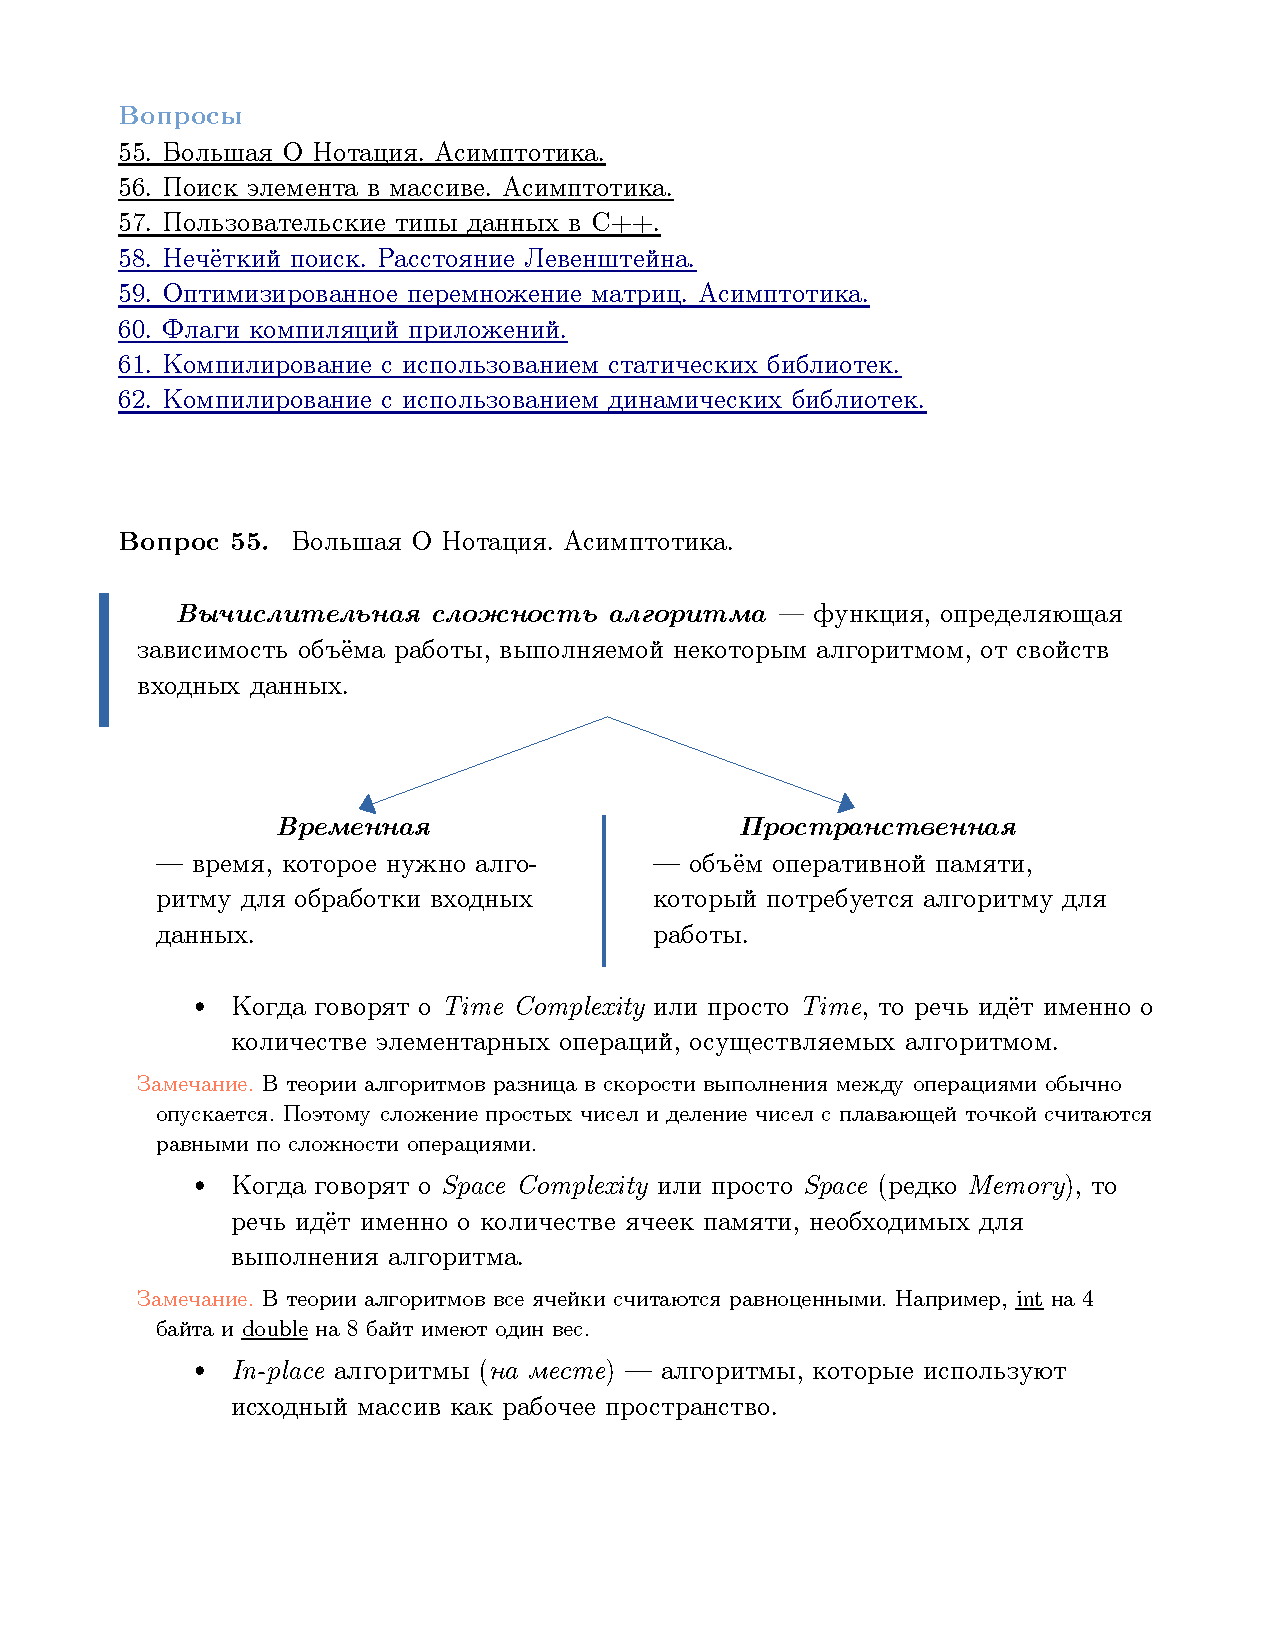
\includepdf[pages=-]{55-62.pdf}

\end{document}